\appendix
\makeatletter\renewcommand\subsection{\@startsection{subsection}{2}{\z@}{1.1ex plus .3ex minus .2ex}{-0.6em}{\normalfont\bfseries}}\makeatother
\makeatletter\renewcommand\p@subsection{\thesection.}\makeatother


% cut-flow table pending together with the last float of the body, so that Fig. XIV, the table and Appendix A share one page
\newpage
\section{Dataset and Preselection}
\label{app:ext_data}
\emph{In short: the branches read by the analysis and the cut flow of the preselection.}
\subsection{Branches and Preselection}
\label{app:branches}
\emph{In short: the analysis reads momentum, particle-identification likelihoods, muon flag and charge of each track; the common preselection keeps $23{,}895$ candidates ($0.28\%$), mostly through the kaon-identification requirement.}

\subsection{Cut Flow of the Preselection}
\label{app:cutflow}
\emph{In short: the kaon-identification requirement on the three tracks is by far the most selective (Table~\ref{tab:cutflow}).}

Table~\ref{tab:cutflow} gives the number of candidates passing each requirement alone and cumulatively, by magnet polarity.

\FloatBarrier

\section{Mass Model and Likelihood}
\label{app:model}
\emph{In short: the relation between the extended likelihood and a mixture with fixed total.}
\subsection{Extended Likelihood versus a Mixture with Fixed Total}
\label{app:ext_mixture}
\emph{In short: the extended form differs from a mixture with fixed total only by the Poisson term of the total yield, which carries no information on $A$; the purity of the signal window is about $96\%$.}

\FloatBarrier

\section{Frequentist Analysis}
\label{app:freq}
\emph{In short: why the Hesse matrix and the significance $Z=\sqrt{q(0)}$ follow from the likelihood, the Neyman construction, and the uncertainties of the twelve parameters by three methods.}
\subsection{Hesse Uncertainties, Test of $A=0$ and Significance}
\label{sec:appendix_freq}
\emph{In short: the Hesse matrix is the inverse of the Fisher information, the test statistic is the profile likelihood ratio, and the significance is $Z=\sqrt{q(0)}$.}
\emph{Why $Z=\sqrt{q(0)}$.} Let $\theta$ be all the parameters, $\hat\theta$ the maximum-likelihood estimate and $I$ the Fisher information. Near the maximum the log-likelihood is parabolic,
\[
-2\ln L(\theta)\simeq-2\ln L(\hat\theta)+(\theta-\hat\theta)^{T}I\,(\theta-\hat\theta),
\]
so asymptotically $\hat\theta$ is Gaussian with covariance $V=I^{-1}$: this is the Hesse matrix, and $\sigma(A)=\sqrt{V_{AA}}$ already includes the effect of the other parameters. For the null hypothesis $A=0$ the statistic is the profile likelihood ratio $q(0)=-2\ln\big[L(0,\hat{\hat\theta})/L(\hat A,\hat\theta)\big]$. For a parabolic likelihood, maximizing over the other parameters at fixed $A$ gives
\[
q(0)=\frac{\hat A^{2}}{V_{AA}}=\Big(\frac{\hat A}{\sigma(A)}\Big)^{2},
\]
and under $H_0$ the variable $\hat A/\sigma(A)$ is a standard normal $N$. Hence $q(0)=N^{2}\sim\chi^{2}_{1}$: one degree of freedom, the parameter fixed by $H_0$, whatever the number of the others. This is Wilks' theorem, exact for a parabolic likelihood and an approximation otherwise. The $p$-value is then
\[
p=P(\chi^{2}_{1}\geq q_{\mathrm{obs}})=P\big(|N|\geq\sqrt{q_{\mathrm{obs}}}\big)=2\big[1-\Phi(\sqrt{q_{\mathrm{obs}}})\big],
\]
which is the probability of a normal variable beyond $\sqrt{q}$ standard deviations: $Z=\sqrt{q(0)}$ is the significance in units of $\sigma$ (two-sided). With $q\simeq27$, $p=2.05\times10^{-7}$ and $Z=5.20$; the one-sided convention $\Phi^{-1}(1-p)$ would give $5.06$, and the Hesse ratio $|\hat A|/\sigma(A)=5.19$ coincides with $\sqrt q$ because the likelihood is nearly parabolic. The approximation fails if the sample is small or $A$ is near a boundary of its range.

\subsection{Neyman Construction and Dependence on the Momentum}
\label{sec:checks_belt}
\emph{In short: inverting the test of $A_{\mathrm{true}}$ with toy-MC experiments gives the same interval as the likelihood ratio (Fig.~\ref{fig:checks_belt}), and $\Araw$ does not depend on the momentum of the $B$ (Table~\ref{tab:checks_momentum}, Fig.~\ref{fig:momentum_terciles}).}

Figure~\ref{fig:checks_belt} shows the central $68\%$ and $95\%$ ranges of $\hat A$ for each $A_{\mathrm{true}}$: the interval is read where the observed $\hat A$ crosses the $68\%$ band.

Table~\ref{tab:checks_momentum} gives $\Araw$ in terciles of the transverse momentum and of the momentum of the $B$ candidate.

Figure~\ref{fig:momentum_terciles} shows the same values in terciles of (a) the transverse momentum and (b) the momentum, against the global value and its $\pm1\sigma$ band.

\begin{figure*}[!t]
\centering
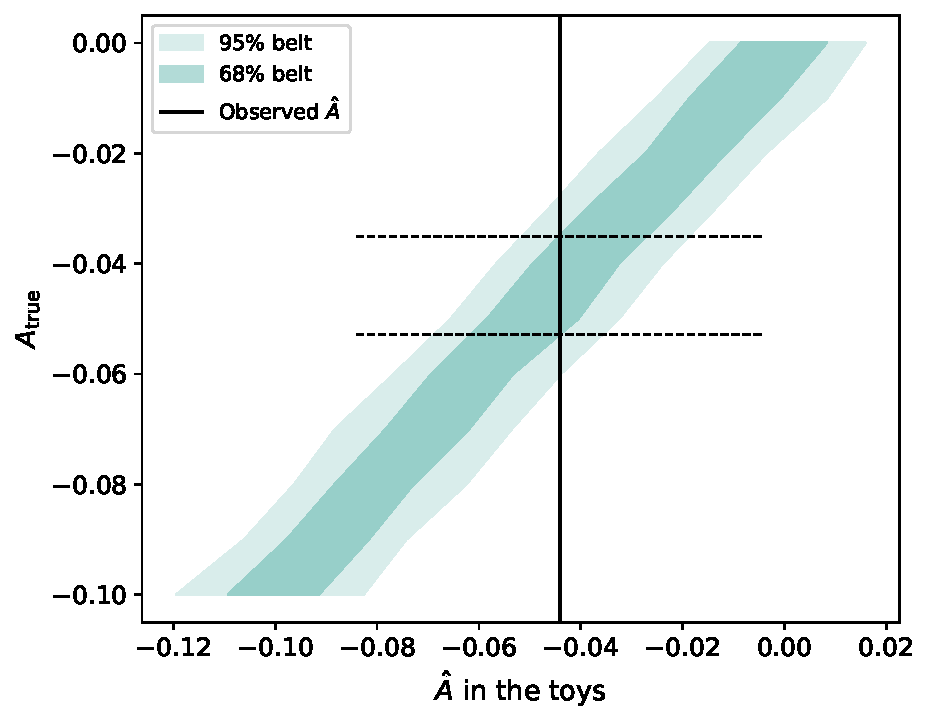
\includegraphics[width=0.5\textwidth]{figures/validation_neyman_belt.pdf}
\caption{Confidence belt of $\hat A$ from toy-MC experiments (central $68\%$ and $95\%$ ranges) as a function of $A_{\mathrm{true}}$; the vertical line is the observed $\hat A$ and the dashed lines the resulting $68\%$ interval.}
\label{fig:checks_belt}
\end{figure*}




\begin{figure*}[!t]
\makeatletter\def\@captype{table}\makeatother
\centering
\begin{tabular}{lccc}
\toprule
Bin & range [GeV] & $n$ & $\Araw$ \\
\midrule
$p_T$, 1 & $1.0$--$4.7$ & $6577$ & $-0.0563\pm0.0169$ \\
$p_T$, 2 & $4.7$--$8.2$ & $6577$ & $-0.0362\pm0.0141$ \\
$p_T$, 3 & $8.2$--$30.5$ & $6577$ & $-0.0452\pm0.0134$ \\
$p$, 1 & $26.7$--$78.1$ & $6577$ & $-0.0391\pm0.0139$ \\
$p$, 2 & $78.1$--$110.1$ & $6577$ & $-0.0475\pm0.0149$ \\
$p$, 3 & $110.1$--$288.5$ & $6577$ & $-0.0478\pm0.0153$ \\
\bottomrule
\end{tabular}
\caption{$\Araw$ (joint frequentist fit) in terciles of the transverse momentum and of the momentum of the $B$ candidate.}
\label{tab:checks_momentum}
\end{figure*}

\begin{figure*}[!t]
\centering
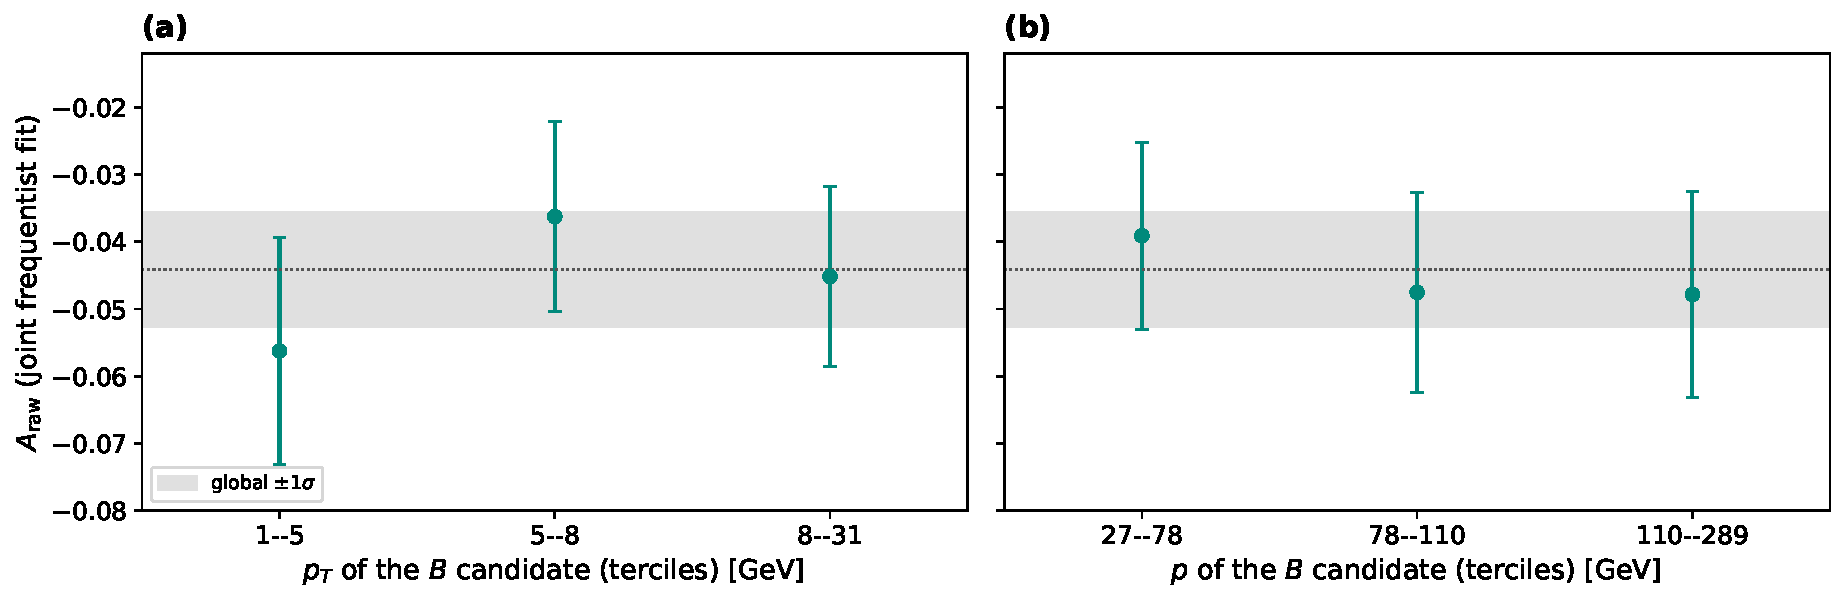
\includegraphics[width=0.85\textwidth]{figures/momentum_terciles.pdf}
\caption{$\Araw$ (joint frequentist fit) in terciles of (a) the transverse momentum and (b) the momentum of the $B$ candidate, with the global value and its $\pm1\sigma$ band; each bin has $6577$ candidates.}
\label{fig:momentum_terciles}
\end{figure*}

\subsection{Uncertainties of the Twelve Parameters by Three Methods}
\label{sec:checks_covariance}
\emph{In short: the inverse of the Fisher information (Hesse), the bootstrap of the data and the posterior give the same standard deviations for $A$, $A_b$, $\mu$ and $\sigma$ (Table~\ref{tab:checks_covariance}, Fig.~\ref{fig:uncertainties_12}); the bootstrap differs for the two yields, because it keeps the total number of candidates fixed, and for the steep slope $\lambda_1^+$, which is weakly constrained.}

Table~\ref{tab:checks_covariance} lists the standard deviation of each parameter of the nominal fit by the three methods.

Figure~\ref{fig:uncertainties_12} shows the standard deviations from the bootstrap ($300$ replicas) and from the posterior divided by the Hesse uncertainty, with a $\pm10\%$ band.

\begin{figure*}[!t]
\makeatletter\def\@captype{table}\makeatother
\centering
\begin{tabular}{lccc}
\toprule
Parameter & Hesse & Bootstrap & Posterior \\
\midrule
$A$ & $0.0085$ & $0.0085$ & $0.0085$ \\
$A_b$ & $0.0177$ & $0.0183$ & $0.0176$ \\
$N_s$ & $133$ & $72$ & $133$ \\
$N_b$ & $82$ & $72$ & $82$ \\
$\mu$ [MeV] & $0.159$ & $0.159$ & $0.161$ \\
$\sigma$ [MeV] & $0.141$ & $0.150$ & $0.138$ \\
$\lambda_1^+$ & $0.0077$ & $0.0057$ & $0.0078$ \\
$\lambda_2^+$ & $0.00028$ & $0.00030$ & $0.00029$ \\
$f_+$ & $0.028$ & $0.029$ & $0.030$ \\
$\lambda_1^-$ & $0.0047$ & $0.0043$ & $0.0047$ \\
$\lambda_2^-$ & $0.00040$ & $0.00038$ & $0.00039$ \\
$f_-$ & $0.039$ & $0.036$ & $0.037$ \\
\bottomrule
\end{tabular}
\caption{Standard deviation of the parameters of the nominal fit from the Hesse matrix, from the bootstrap of the data and from the posterior.}
\label{tab:checks_covariance}
\end{figure*}


\begin{figure*}[!t]
\centering
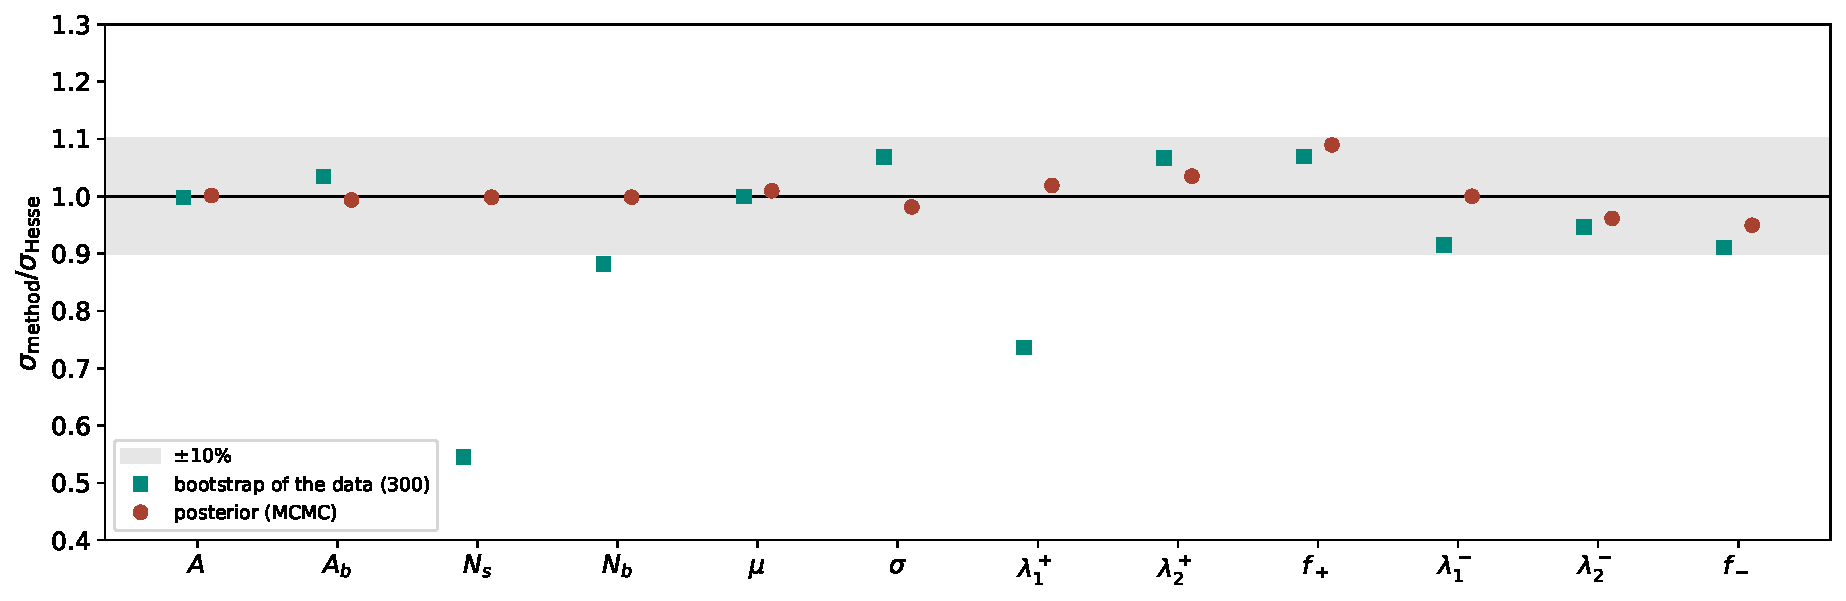
\includegraphics[width=0.85\textwidth]{figures/uncertainties_12.pdf}
\caption{Standard deviation of the twelve parameters of the nominal fit from the bootstrap of the data ($300$ replicas) and from the posterior, divided by the Hesse uncertainty; the band is $\pm10\%$.}
\label{fig:uncertainties_12}
\end{figure*}

\section{Bayesian Analysis}
\label{app:ext_bayes}
\emph{In short: the prior sensitivity, the sampler and its trace plots, the derivation of the Savage-Dickey ratio, the intervals, the model-adequacy checks, the magnet-polarity check, the toy-MC coverage of the credible interval and the tabulated profile likelihood.}
\subsection{Priors and Bayes Factors}
\label{sec:checks_prior}
\emph{In short: no change of the prior on the nuisance parameters or of its parametrization moves $A$ by more than $0.0002$ (Table~\ref{tab:checks_prior}); the Bayes factor of $A=0$ scales with the prior width (Fig.~\ref{fig:checks_bf}), and the evidence computed by direct integration agrees in order of magnitude with the Savage-Dickey ratio.}

Table~\ref{tab:checks_prior} gives the posterior of $A$ under the alternative priors, with the effective sample size of the reweighted chain.

Figure~\ref{fig:checks_bf} shows $BF_{01}$ of $A=0$ and of $A_b=0$ against the half-width of the uniform prior, with the nominal prior marked.


\subsection{Sampling the Posterior}
\label{app:theory}
\emph{In short: Metropolis-Hastings accepts a proposal with a ratio that satisfies detailed balance; the affine-invariant ensemble move samples correlated posteriors without tuning, and $N/\tau$ is the effective length of a chain.}

\subsection{Trace Plots of the Walkers}
\label{sec:appendix}
\emph{In short: walkers started over the whole prior box converge to the same mode (Fig.~\ref{fig:bayes_trace}).}

Figure~\ref{fig:bayes_trace} shows the trace of $A$, $N_s$, $\sigma$ and $f_+$ for the $32$ walkers: the first $3000$ steps over the full range, and the whole chain zoomed on the posterior with the burn-in marked.


\subsection{Published Profile Likelihood}
\label{sec:checks_mh}
\emph{In short: the profile likelihood ratio $q(A)$ of the nominal fit is tabulated (Table~\ref{tab:checks_qa}), so that the result can be combined with others.}

Table~\ref{tab:checks_qa} gives $q(A)$ for $A$ between $-0.08$ and $0$, with the minimum and the Minos intervals of the nominal fit (other parameters profiled).

\subsection{Model Adequacy: Goodness of Fit and Posterior Predictive Check}
\label{sec:bayes_gof}
\emph{In short: the model does not reach $\chi^2/\mathrm{ndof}\approx1$ ($164.1/88$), mainly because the signal tails are heavier than a Gaussian, but $\Araw$ changes by only $-0.0002$ with a Crystal Ball signal (Table~\ref{tab:gof}); the pulls of the mass fit are in Fig.~\ref{fig:bayes_fit}.}

Table~\ref{tab:gof} compares $\Araw$ and the goodness of fit of the nominal model with those of the alternative signal and background models, on the same data.

Figure~\ref{fig:bayes_ppc} shows the posterior predictive distributions of (a) the binned $\chi^2$ and of the counting asymmetry of (b) the fit window and (c) the sidebands, against the observed values.

Figure~\ref{fig:bayes_fit} shows the mass distributions of (a) $B^+$ and (b) $B^-$ candidates with the nominal model, and the pulls below.


\subsection{Savage--Dickey Ratio}
\label{sec:appendix_sd}
\emph{In short: the Bayes factor of $A=0$ is the ratio of the posterior and prior densities at $A=0$, with no integral over the twelve parameters.}

\emph{Proof.} Write $\theta$ for the parameters other than $A$. Let $H_1$ have $A$ free with the prior $\pi(A,\theta)=\pi(A)\,\pi(\theta)$, and let $H_0$ be $H_1$ with $A=0$ and the same $\pi(\theta)$. The evidence of $H_0$ is
\[
P(D\mid H_0)=\int \mathcal{L}(D\mid A=0,\theta)\,\pi(\theta)\,d\theta ,
\]
and that of $H_1$ is $P(D\mid H_1)=\int\!\!\int \mathcal{L}(D\mid A,\theta)\,\pi(A)\,\pi(\theta)\,dA\,d\theta$. The marginal posterior density of $A$ in $H_1$, evaluated at $A=0$, is obtained by Bayes' theorem and by integrating over $\theta$:
\[
p(A=0\mid D)=\int \frac{\mathcal{L}(D\mid A=0,\theta)\,\pi(A=0)\,\pi(\theta)}{P(D\mid H_1)}\,d\theta
=\pi(A=0)\,\frac{P(D\mid H_0)}{P(D\mid H_1)} .
\]
Dividing by $\pi(A=0)$ gives
\[
BF_{01}=\frac{P(D\mid H_0)}{P(D\mid H_1)}=\frac{p(A=0\mid D)}{\pi(A=0)} .
\]
It holds only if $A$ and $\theta$ are independent a priori and the other priors are shared by the two hypotheses; the priors must be proper (here $\pi(A=0)=\tfrac12$), otherwise the Bayes factor is not defined.

\subsection{Equal-Tailed and Highest-Posterior-Density Intervals}
\label{sec:checks_hpd}
\emph{In short: for $A$ and $A_b$ the two kinds of $68\%$ interval coincide; they differ for the skewed parameters, whose highest-posterior-density interval is shifted towards the mode (Table~\ref{tab:checks_hpd}).}
Table~\ref{tab:checks_hpd} lists, for each parameter, the equal-tailed and highest-posterior-density $68\%$ intervals and the skewness of the marginal posterior.


\subsection{Posterior Predictive Check with Statistics Not Fitted by the Model}
\label{sec:checks_ppc}
\emph{In short: the asymmetry in slices of the mass, which the model predicts, is reproduced ($p_B=0.67$, Fig.~\ref{fig:checks_ppc}b), and the difference between the $\chi^2$ of the two charges is at the edge of the replicas ($p_B=0.08$, Fig.~\ref{fig:checks_ppc}c).}

Figure~\ref{fig:checks_ppc} shows (a) the counting asymmetry in slices of $50\,\MeV$ of the mass, data and model, (b) the distribution of $T=\sum_s(A_s-\bar A_s)^2/\sigma_s^2$ over $1000$ replicas with the observed value, and (c) the same for $\chi^2(B^+)-\chi^2(B^-)$.

\subsection{Robustness Check: Magnet Polarity}
\label{sec:bayes_checks}
\emph{In short: the posteriors of $\Araw$ for the magnet-down and magnet-up samples and for their combination agree within $0.7\sigma$ (Fig.~\ref{fig:bayes_magnet}).}

Figure~\ref{fig:bayes_magnet} shows the posterior of $\Araw$ for the magnet-down, magnet-up and combined samples.


\subsection{Toy-MC Coverage Validation}
\label{sec:bayes_toymc}
\emph{In short: $200$ toy-MC experiments give coverage $0.65\pm0.03$ ($68\%$) and $0.93\pm0.02$ ($95\%$) (Fig.~\ref{fig:bayes_toys}b), consistent with nominal, with unbiased estimates and pulls of width $1.04$ (Fig.~\ref{fig:bayes_toys}a).}

Figure~\ref{fig:bayes_toys} shows (a) the pulls of the posterior median and standard deviation of each replica against a standard normal, and (b) the fraction of replicas whose $68\%$ and $95\%$ credible intervals contain the injected value, with binomial uncertainties.

\FloatBarrier
% ---- figures and tables of this appendix, in the order in which they are cited ----
\begin{table}[h]
\centering
\resizebox{\ifdim\width>\linewidth\linewidth\else\width\fi}{!}{\begin{tabular}{lccc}
\toprule
Prior & $A$ (median) & $68\%$ interval & ESS \\
\midrule
Nominal (uniform) & $-0.0442$ & $[-0.0529,-0.0358]$ & $20000$ \\
Log-uniform $N_s$, $N_b$ & $-0.0442$ & $[-0.0529,-0.0358]$ & $19993$ \\
Log-uniform slopes & $-0.0440$ & $[-0.0528,-0.0356]$ & $12306$ \\
Uniform in $1/\lambda$ & $-0.0444$ & $[-0.0526,-0.0360]$ & $153$ \\
Flat in $(N_s^+,N_s^-)$ & $-0.0442$ & $[-0.0529,-0.0358]$ & $19999$ \\
Flat in $(N_s^\pm)$ and $(N_b^\pm)$ & $-0.0442$ & $[-0.0529,-0.0358]$ & $19993$ \\
\bottomrule
\end{tabular}}
\caption{Posterior of $A$ under alternative priors, by importance reweighting of the chain; ESS: effective sample size of the $20{,}000$ thinned samples.}
\label{tab:checks_prior}
\end{table}
\begin{figure*}[!t]
\centering
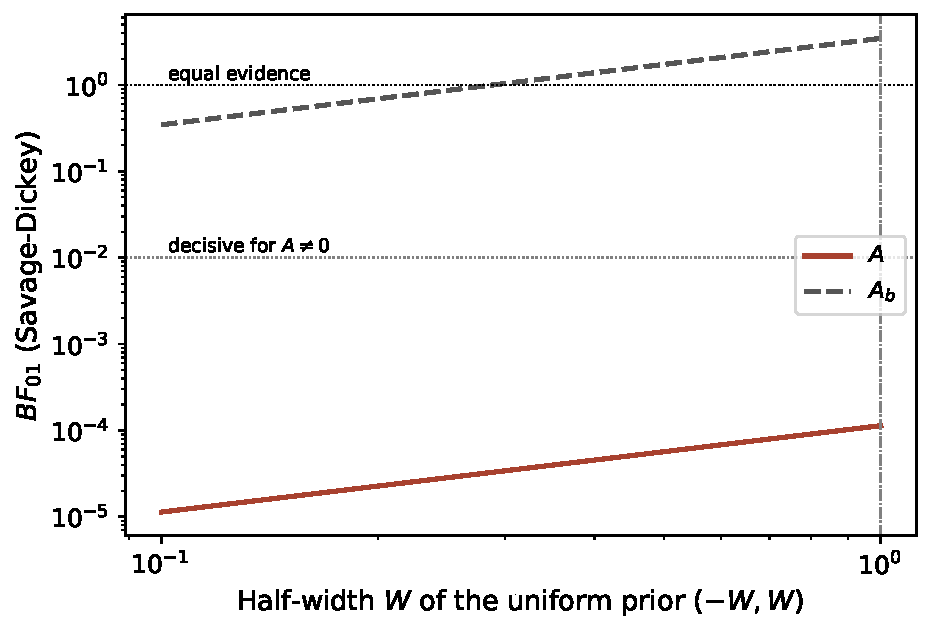
\includegraphics[width=0.5\textwidth]{figures/validation_bf_prior_width.pdf}
\caption{$BF_{01}$ of $A=0$ and of $A_b=0$ as a function of the half-width $W$ of the uniform prior $(-W,W)$ (Gaussian approximation of the posterior, Savage-Dickey). The vertical line marks the nominal prior.}
\label{fig:checks_bf}
\end{figure*}
\begin{figure*}[t]
\centering
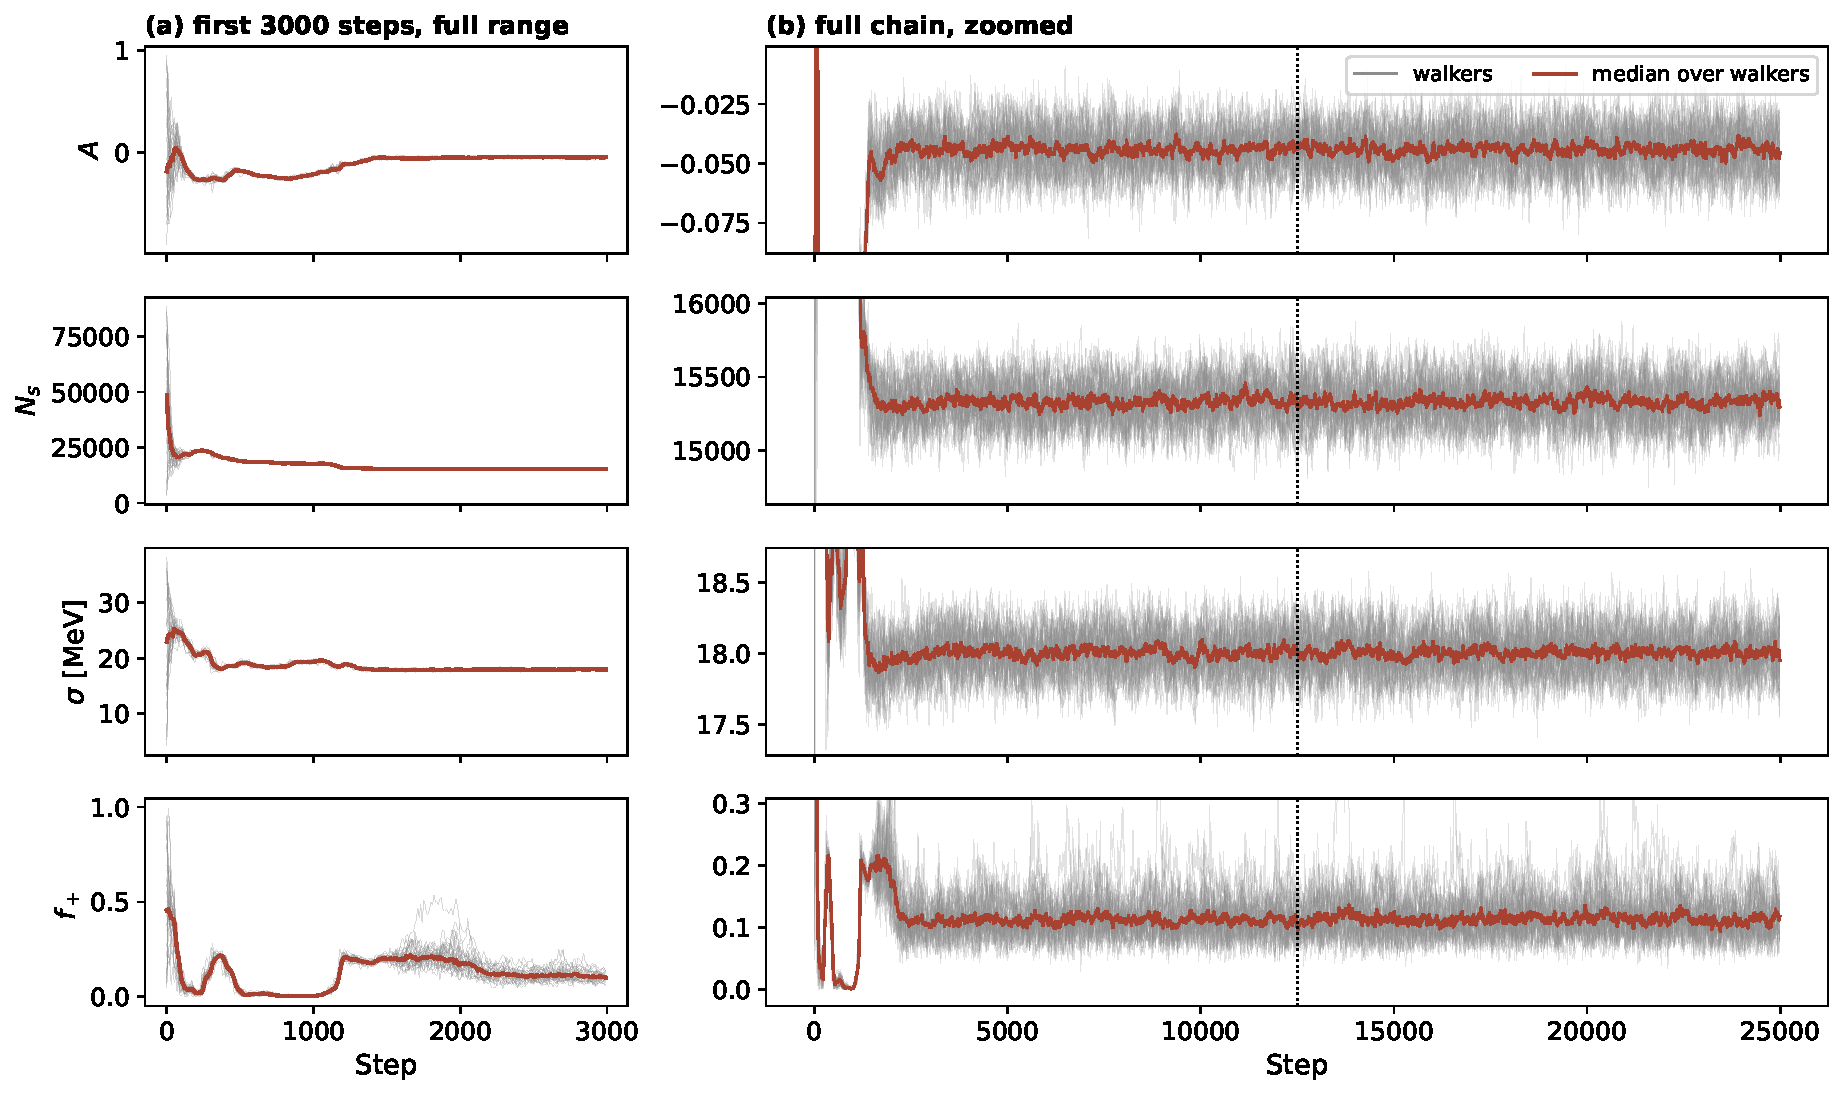
\includegraphics[width=0.7\textwidth]{figures/bayes_nominal_trace.pdf}
\caption{Trace plot of the nominal fit with the 32 walkers initialized uniformly over the prior box (one grey line per walker, every 10th step; colored: median over the walkers), for $A$, $N_s$, $\sigma$ and the steep-background fraction $f_+$. Left: first 3000 steps, full range; right: whole chain, zoomed on the posterior. The first half of the chain (dotted line) is discarded as burn-in.}
\label{fig:bayes_trace}
\end{figure*}
% magnet posteriors, toy-MC validation and q(A) table in one float page, evenly spaced (equal gaps above, between and below)
\begin{figure*}[!p]
\vbox to 0.97\textheight{%
\vfill
\centering
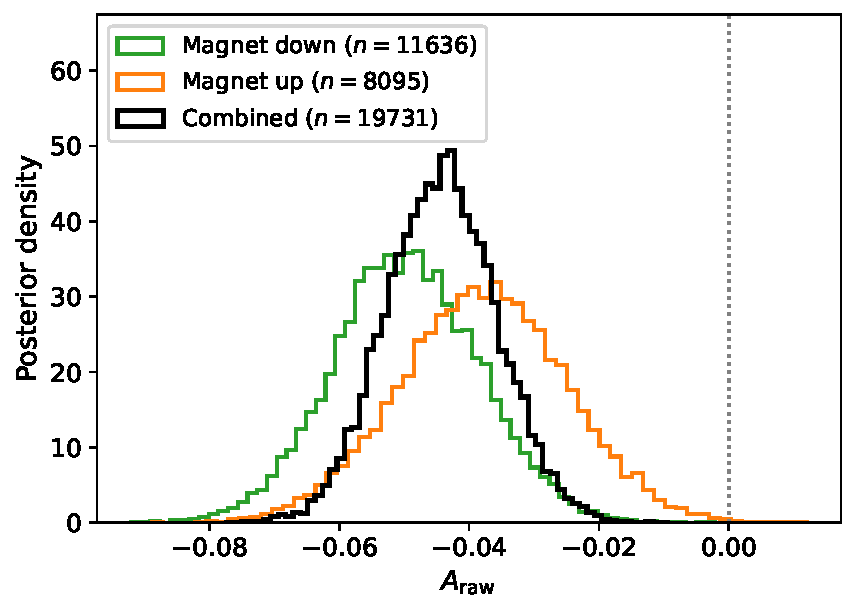
\includegraphics[width=0.5\textwidth]{figures/bayes_nominal_magnet.pdf}
\caption{Posterior of $\Araw$ for the magnet-down, magnet-up and combined samples.}
\label{fig:bayes_magnet}
\vfill
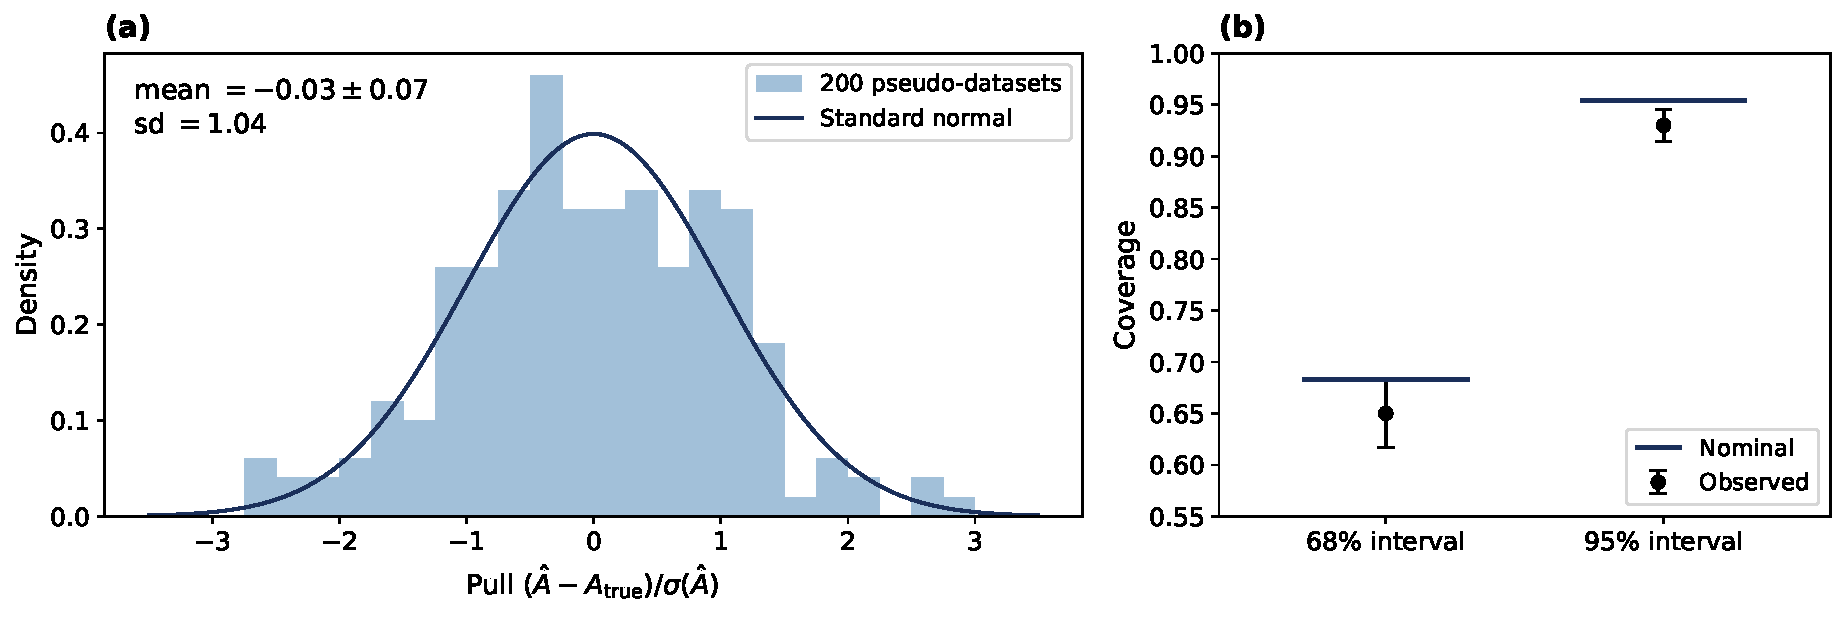
\includegraphics[width=0.8\textwidth]{figures/bayes_nominal_toys.pdf}
\caption{Toy-MC validation, 200 toy-MC datasets. (a) Pulls $(\hat A-A_{\mathrm{true}})/\sigma(\hat A)$, with $\hat A$ and $\sigma(\hat A)$ the posterior median and standard deviation of each replica, compared with a standard normal. (b) Fraction of replicas whose 68\% and 95\% credible intervals contain the injected value, with binomial uncertainties, and the nominal coverage.}
\label{fig:bayes_toys}
\vfill
\makeatletter\def\@captype{table}\makeatother
\resizebox{\ifdim\width>\linewidth\linewidth\else\width\fi}{!}{\begin{tabular}{r|ccccccccc}
\toprule
$A$ & $-0.08$ & $-0.07$ & $-0.06$ & $-0.05$ & $-0.04$ & $-0.03$ & $-0.02$ & $-0.01$ & $+0.00$ \\
$q(A)$ & $17.9$ & $9.3$ & $3.5$ & $0.5$ & $0.2$ & $2.8$ & $8.1$ & $16.1$ & $27.0$ \\
\bottomrule
\end{tabular}}
\caption{Profile likelihood ratio $q(A)=-2\Delta\ln L$ of the nominal fit (other parameters profiled); minimum at $-0.0441$, Minos intervals $[-0.0526,-0.0356]$ ($68\%$) and $[-0.0607,-0.0275]$ ($95\%$).}
\label{tab:checks_qa}
\vfill}
\end{figure*}
\begin{table}[!t]
\centering
\begin{tabular}{lccc}
\toprule
Model & $\Araw$ & $\chi^2$/ndof & $p$ \\
\midrule
Nominal & $-0.0443$ & $164.1/88$ & $2\times10^{-6}$ \\
Crystal Ball signal & $-0.0445$ & $131.0/86$ & $1\times10^{-3}$ \\
$\mu$, $\sigma$ per charge & $-0.0443$ & $164.2/86$ & $8\times10^{-7}$ \\
Shared bkg.\ shape & $-0.0480$ & $174.1/91$ & $4\times10^{-7}$ \\
Symmetric bkg.\ ($A_b=0$) & $-0.0471$ & $169.8/89$ & $5\times10^{-7}$ \\
Single exponential & $-0.0480$ & $297.7/92$ & $2\times10^{-23}$ \\
\bottomrule
\end{tabular}
\caption{$\Araw$ (posterior median) and goodness of fit of the nominal model (Gaussian signal, double exponential per charge) and of the alternative signal and background models, same data and window.}
\label{tab:gof}
\end{table}
\begin{figure*}[t]
\centering
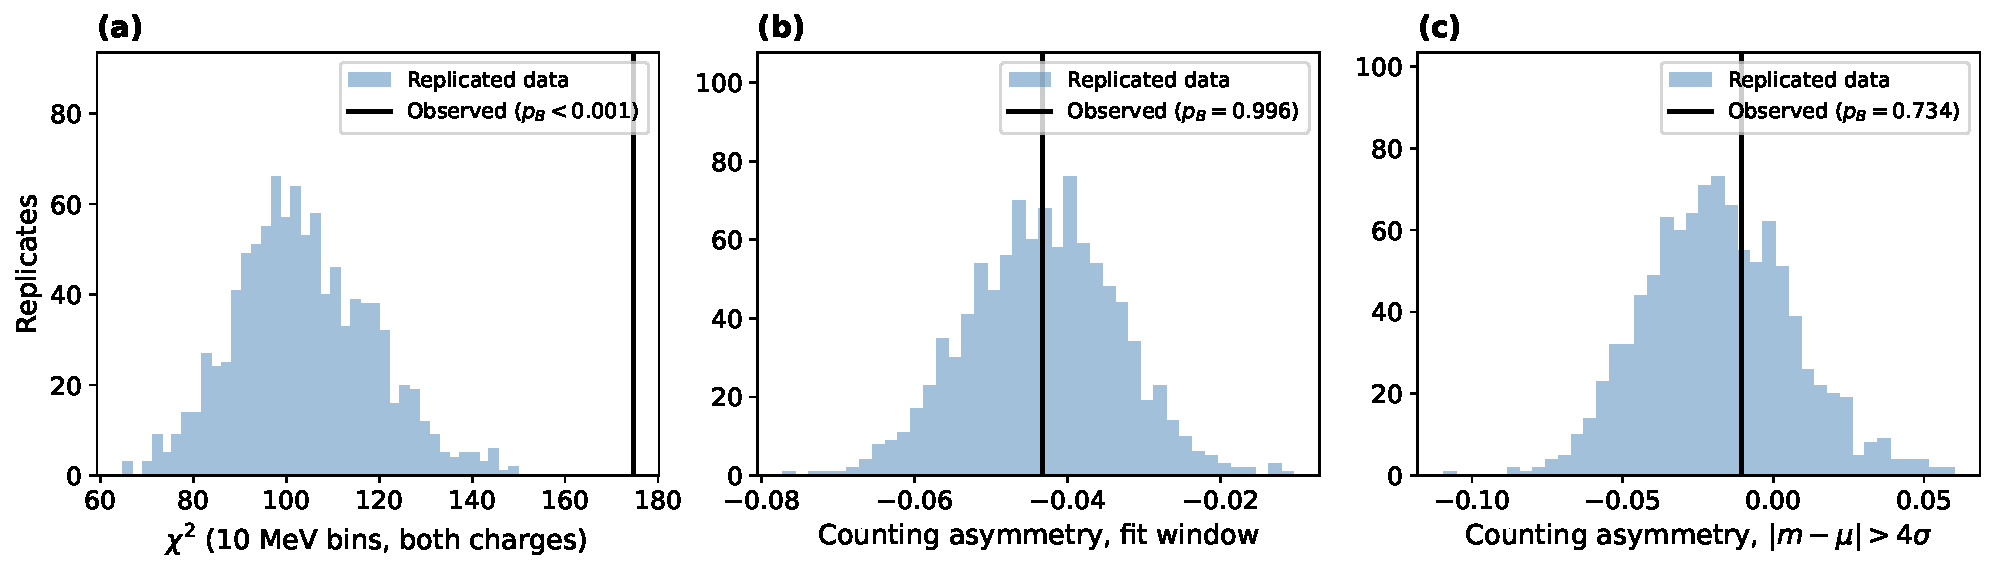
\includegraphics[width=0.7\textwidth]{figures/bayes_nominal_ppc.pdf}
\caption{Posterior predictive check: distributions of three discrepancies over $1000$ datasets replicated from posterior draws, compared with the observed values. (a) binned $\chi^2$; (b) and (c) counting asymmetry of the fit window and of the sidebands.}
\label{fig:bayes_ppc}
\end{figure*}
\begin{figure*}[t]
\centering
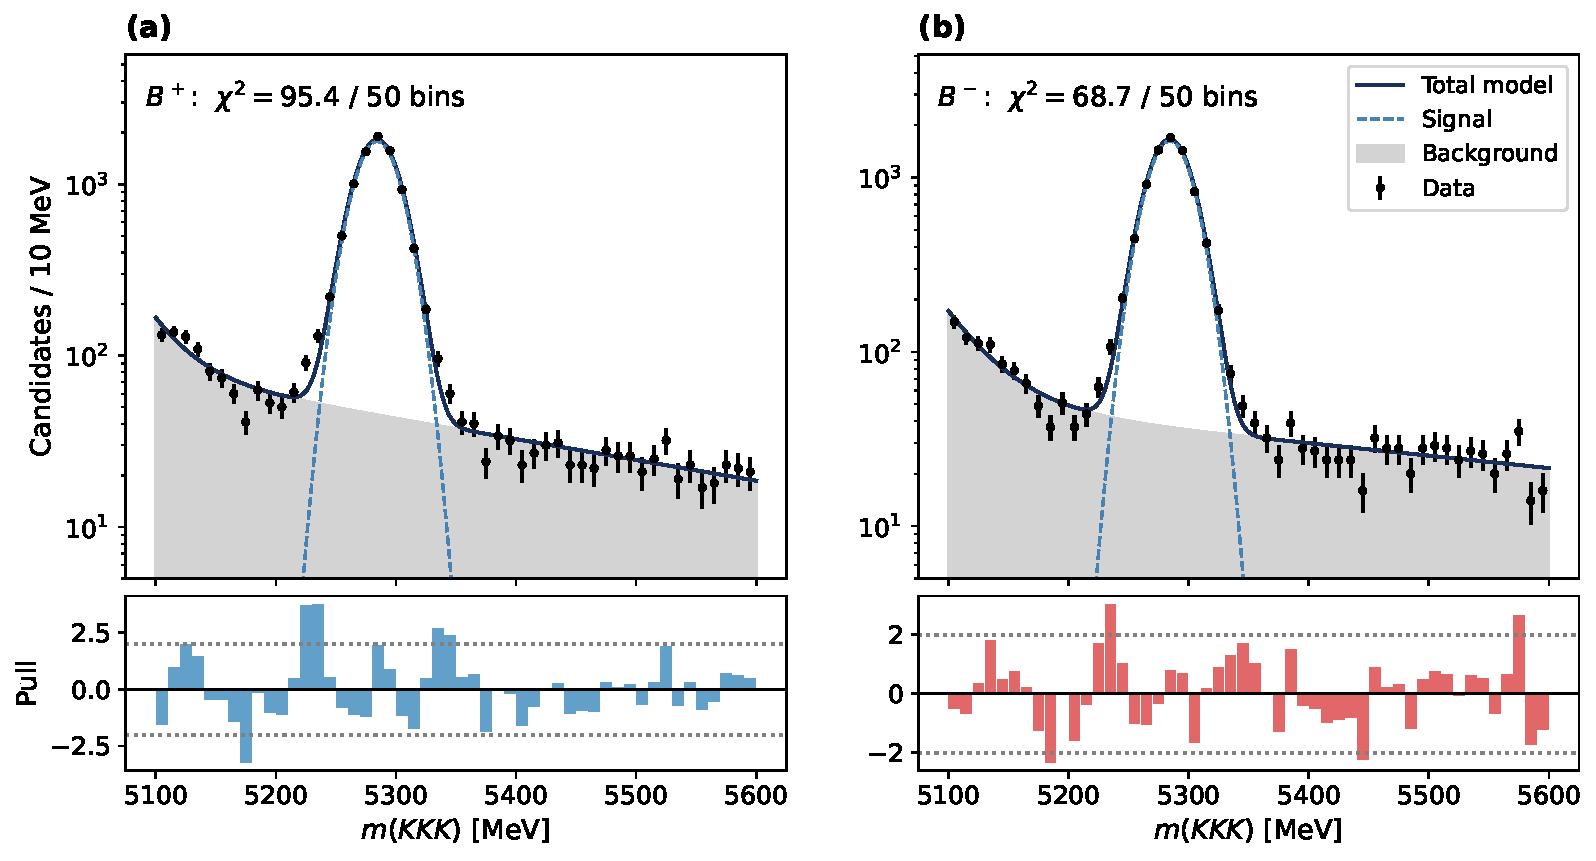
\includegraphics[width=0.7\textwidth]{figures/bayes_nominal_mass_fit.pdf}
\caption{Mass distributions of (a) $B^+$ and (b) $B^-$ candidates with the nominal model (posterior medians, logarithmic scale): total, signal and background components. Bottom: pulls, $(\text{obs}-\text{exp})/\sqrt{\text{exp}}$.}
\label{fig:bayes_fit}
\end{figure*}
\begin{table}[h]
\centering
\resizebox{\ifdim\width>\linewidth\linewidth\else\width\fi}{!}{\begin{tabular}{lcccc}
\toprule
Parameter & median & equal-tailed & HPD & skewness \\
\midrule
$A$ & $-0.0442$ & $[-0.0529,-0.0358]$ & $[-0.0525,-0.0355]$ & $+0.01$ \\
$A_b$ & $-0.0400$ & $[-0.0575,-0.0224]$ & $[-0.0575,-0.0225]$ & $+0.01$ \\
$f_+$ & $0.114$ & $[0.089,0.145]$ & $[0.084,0.138]$ & $+0.90$ \\
$f_-$ & $0.209$ & $[0.174,0.248]$ & $[0.168,0.241]$ & $+0.33$ \\
$\lambda_1^+$ [MeV$^{-1}$] & $0.0350$ & $[0.0281,0.0431]$ & $[0.0274,0.0423]$ & $+0.52$ \\
\bottomrule
\end{tabular}}
\caption{Equal-tailed and highest-posterior-density $68\%$ intervals and skewness of the marginal posteriors.}
\label{tab:checks_hpd}
\end{table}
\begin{figure*}[t]
\centering
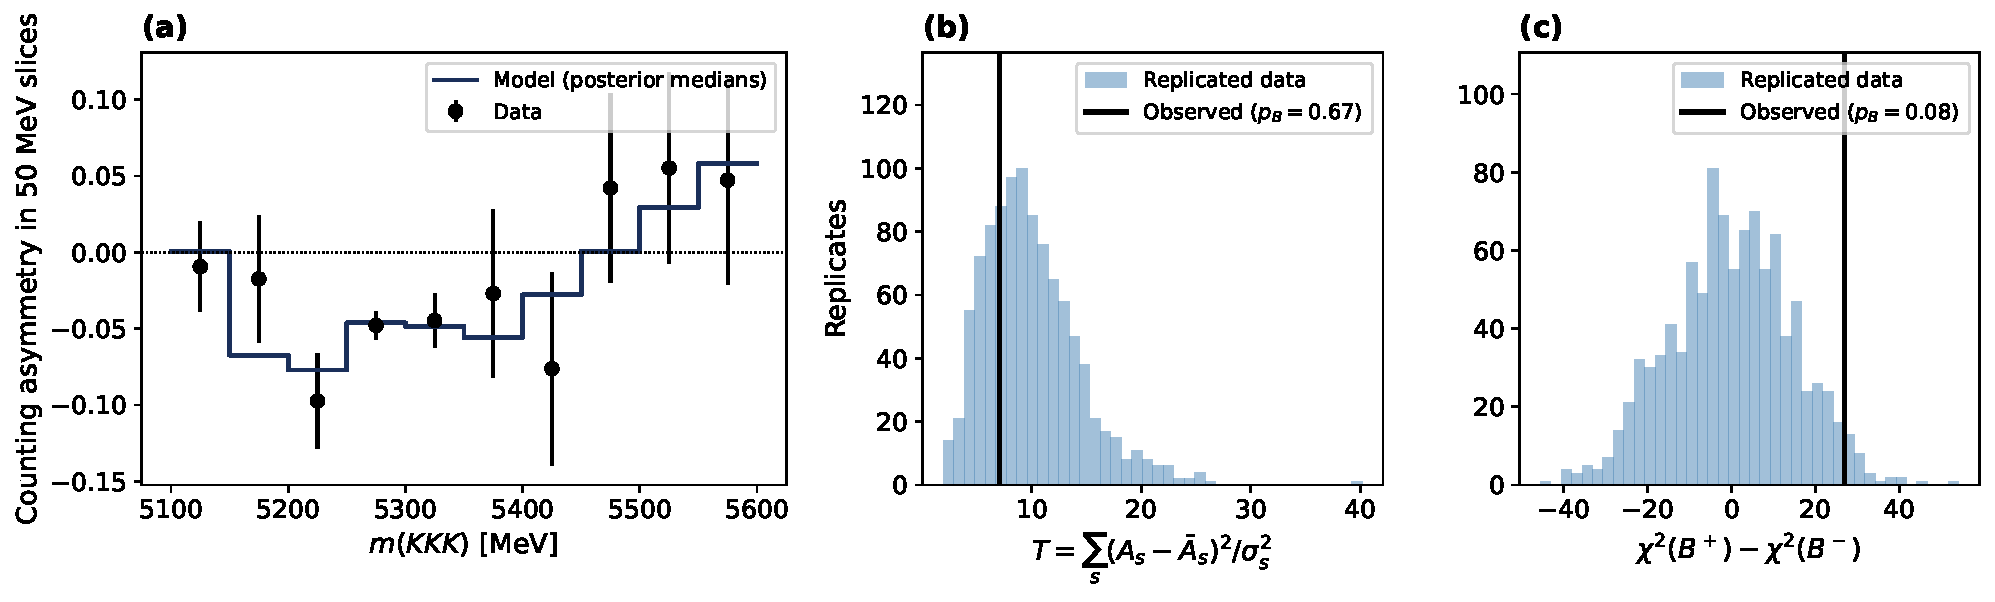
\includegraphics[width=0.7\textwidth]{figures/validation_ppc_unfitted.pdf}
\caption{(a) Counting asymmetry in slices of $50\,\MeV$ of the mass, data and model. (b) Distribution of $T=\sum_s(A_s-\bar A_s)^2/\sigma_s^2$ over $1000$ replicas and observed value. (c) The same for $\chi^2(B^+)-\chi^2(B^-)$.}
\label{fig:checks_ppc}
\end{figure*}

\FloatBarrier

\section{Validation of the Estimator and of the Intervals}
\label{app:ext_valid}
\label{sec:appendix_checks}
\emph{In short: the size and power of the test of $A=0$, the asymptotic behavior of the estimator and the goodness of fit as a function of the binning.}
\subsection{Size and Power of the Test of $A=0$}
\label{sec:validation_power}
\emph{In short: the statistic $q(0)$ follows a $\chi^2$ distribution with one degree of freedom (Fig.~\ref{fig:validation_null}), so the test has the nominal size; an asymmetry of $-0.02$ would be rejected at $3\sigma$ in one toy-MC experiment out of four (Fig.~\ref{fig:validation_injection}c).}

Figure~\ref{fig:validation_null} shows, for toy-MC experiments, (a) the fraction with $q(0)$ above the observed value for $A_{\mathrm{true}}=0$ against the $\chi^2_1$ distribution, (b) the $p$-value of $t(A_{\mathrm{true}})$ against a uniform distribution, at the fitted value and pooled over the injected values, and (c) the distribution of $t(A_{\mathrm{true}})$ at the fitted value against $\chi^2_1$.

\begin{figure*}[!t]
\centering
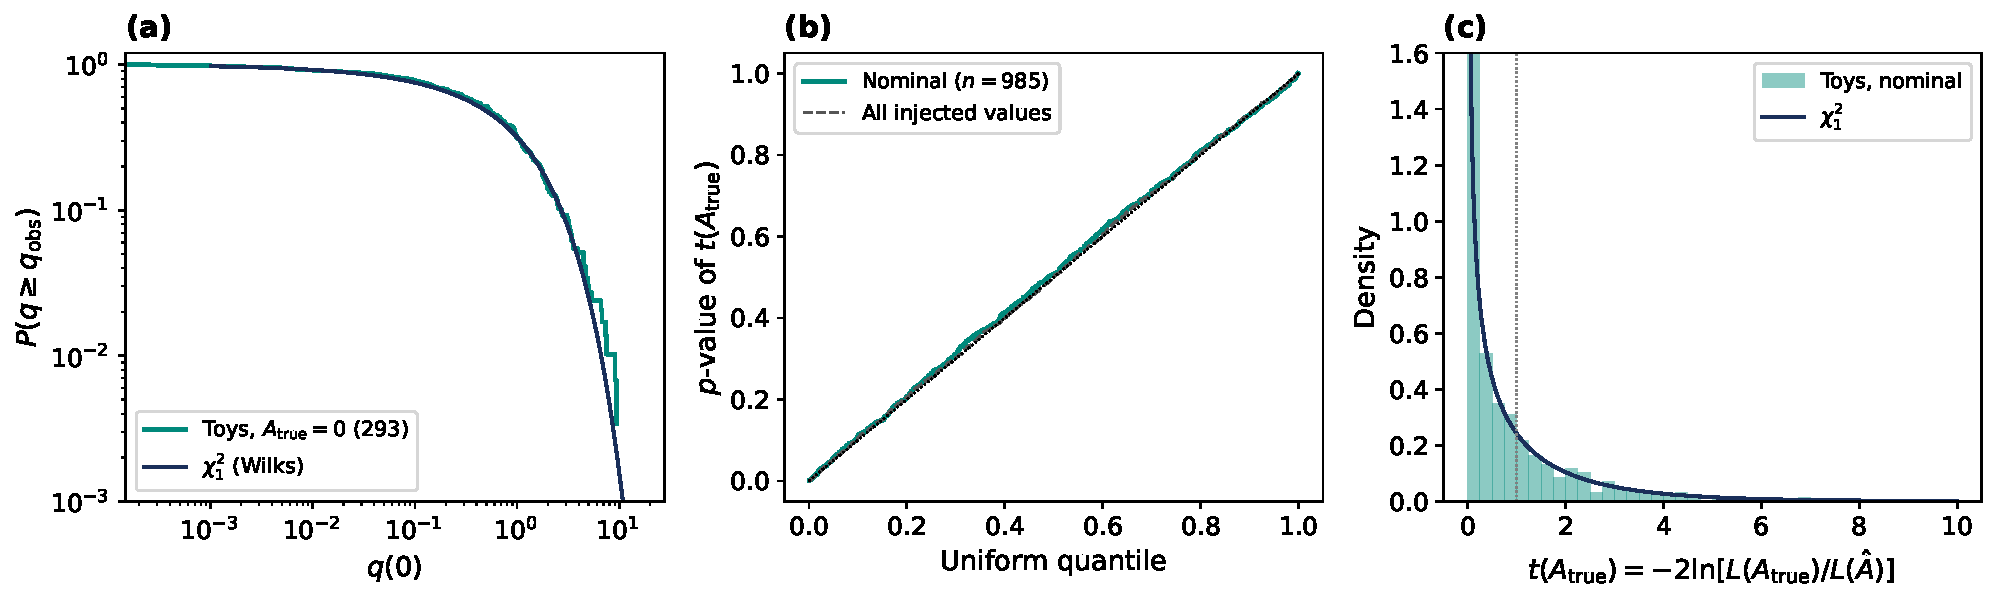
\includegraphics[width=1\textwidth]{figures/validation_null_wilks.pdf}
\caption{Toy-MC experiments, validity of Wilks' theorem. (a) Fraction of experiments with $q(0)$ above the observed value, for $A_{\mathrm{true}}=0$, compared with the $\chi^2_1$ distribution. (b) $p$-value of $t(A_{\mathrm{true}})$ against a uniform distribution, at the fitted value and pooled over the injected values. (c) Distribution of $t(A_{\mathrm{true}})$ at the fitted value and $\chi^2_1$.}
\label{fig:validation_null}
\end{figure*}

\subsection{Asymptotic Behavior of the Estimator}
\label{sec:checks_scaling}
\emph{In short: with the number of candidates the bias tends to zero, the spread scales as $N^{-1/2}$ and the distribution of $\hat A$ becomes Gaussian (Table~\ref{tab:checks_scaling}), as the central limit theorem and the asymptotic properties of the maximum-likelihood estimate predict.}

Table~\ref{tab:checks_scaling} gives, for $N$ from $50$ to $2000$ candidates, the bias, the spread and its product with $\sqrt N$, the skewness, the excess kurtosis and the Shapiro $p$-value of $\hat A$ in $300$ toy-MC datasets.

\begin{figure*}[!t]
\makeatletter\def\@captype{table}\makeatother
\centering
\resizebox{\ifdim\width>\linewidth\linewidth\else\width\fi}{!}{\begin{tabular}{rcccccc}
\toprule
$N$ & bias & sd$(\hat A)$ & sd$\cdot\sqrt N$ & skewness & ex.\ kurtosis & Shapiro $p$ \\
\midrule
$50$ & $-0.0085$ & $0.1611$ & $1.14$ & $-0.15$ & $+0.64$ & $0.03$ \\
$150$ & $-0.0051$ & $0.0920$ & $1.13$ & $+0.16$ & $+0.31$ & $0.59$ \\
$500$ & $-0.0022$ & $0.0501$ & $1.12$ & $-0.08$ & $+0.38$ & $0.52$ \\
$2000$ & $+0.0009$ & $0.0225$ & $1.01$ & $-0.20$ & $-0.20$ & $0.32$ \\
\bottomrule
\end{tabular}}
\caption{Distribution of the maximum-likelihood estimate of $A$ in $300$ toy-MC datasets of $N$ candidates.}
\label{tab:checks_scaling}
\end{figure*}

\subsection{Goodness of Fit and the Binning}
\label{sec:validation_gof}
\emph{In short: the binned $\chi^2$ of toy-MC experiments follows its asymptotic distribution, so its $p$-values are accurate; the misfit of the data is $5.4$ standard deviations at $10\,\MeV$ bins (Fig.~\ref{fig:validation_gof}a) and $2.0$ at $2.5\,\MeV$ (Fig.~\ref{fig:validation_gof}b), because it lives on the scale of the flanks of the peak.}

Figure~\ref{fig:validation_gof} shows the binned $\chi^2$ of $1000$ toy-MC experiments against the $\chi^2$ distribution with the corresponding degrees of freedom, and the value of the data, for (a) $2\times50$ bins of $10\,\MeV$ and (b) $2\times200$ bins of $2.5\,\MeV$.

\begin{figure*}[!t]
\centering
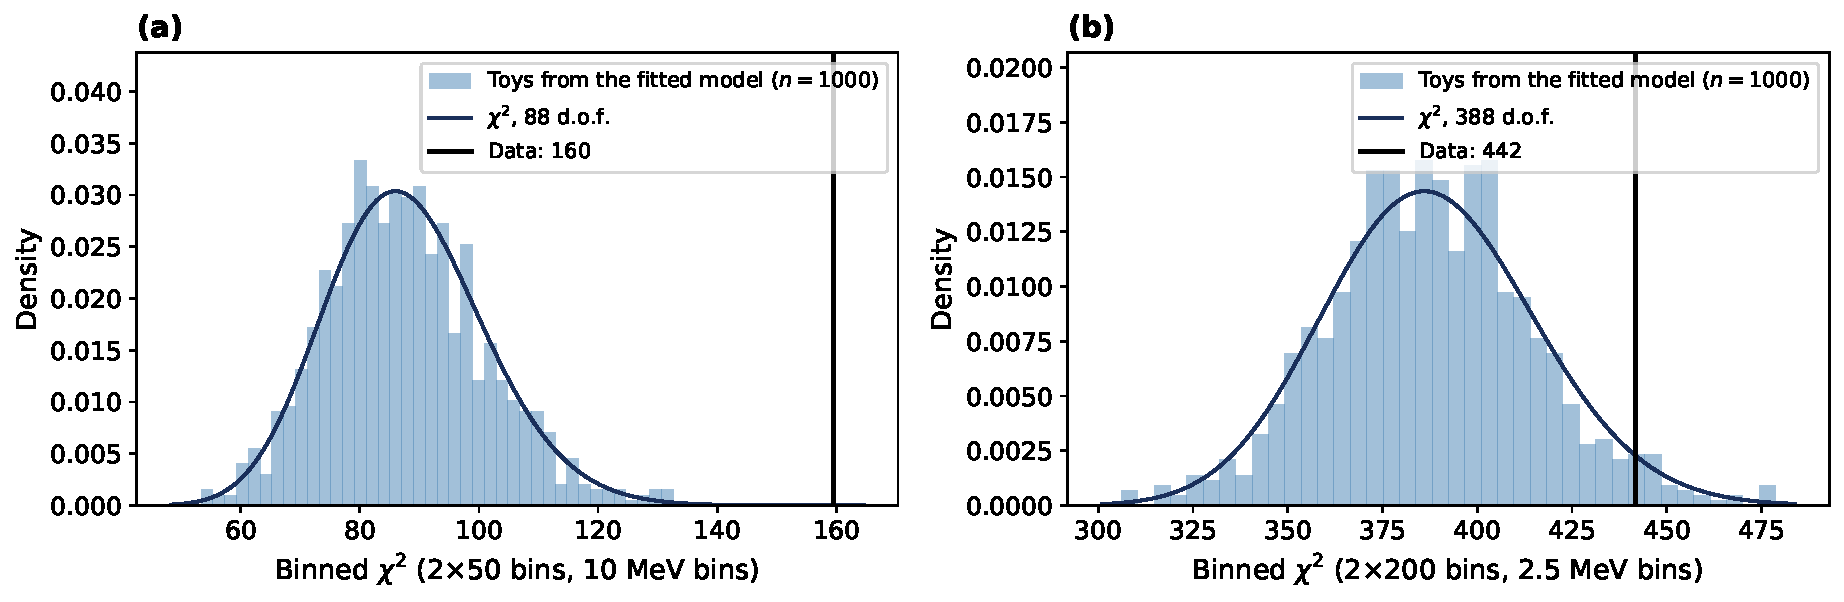
\includegraphics[width=1\textwidth]{figures/validation_gof_toys.pdf}
\caption{Binned $\chi^2$ of $1000$ toy-MC experiments from the fitted model, $\chi^2$ distribution with the corresponding degrees of freedom, and value of the data: (a) $2\times50$ bins of $10\,\MeV$, (b) $2\times200$ bins of $2.5\,\MeV$.}
\label{fig:validation_gof}
\end{figure*}

\FloatBarrier

\section{Machine-Learning Analysis}
\label{sec:ml}
\emph{In short: classifiers trained on weak labels from the mass spectrum (there are no true labels) reach a test AUC of $0.86$; a cut on their score leaves $\Araw$ unchanged, and an adaptive partition of the Dalitz plane shows the same pattern as the fixed binning.}
\subsection{Background: Regularization, Bias-Variance and Loss Functions}
\label{app:theory_ml}
\emph{In short: cross-entropy is a Bernoulli negative log-likelihood, $L1$ and $L2$ penalties shrink the coefficients, the test error splits into bias, variance and noise, and class weights rescale the score by a known factor.}

\subsection{Background: Clustering and Uncertainty Estimators}
\label{app:theory_cluster}
\emph{In short: $K$-means converges to a local minimum of the inertia, the adjusted Rand index measures the stability of a partition, and the spread of an ensemble estimates the epistemic uncertainty.}

\subsection{Model Comparison}
\label{sec:ml_models}
\emph{In short: six classifiers; the tree ensembles and the neural network reach test AUC $0.857$--$0.864$, about $0.09$ above the linear models and indistinguishable from each other within the test-set uncertainty ($0.012$; Table~\ref{tab:ml_models}, Fig.~\ref{fig:ml_roc}a); gradient boosting, best in cross-validation, is the reference.}

Table~\ref{tab:ml_models} gives the cross-validated AUC, the test-set AUC with its bootstrap uncertainty and the Brier score of each model.

Figure~\ref{fig:ml_roc} shows (a) the ROC curves and (b) the significance improvement of a cut on the score against the signal-like efficiency.

Figure~\ref{fig:ml_features} compares (a) the Random Forest feature importance with (b) the magnitude of the Lasso coefficients.

\subsection{Regularization, Bias-Variance, and Calibration}
\label{sec:ml_regcal}
\emph{In short: the linear model does not overfit (Fig.~\ref{fig:ml_regularization}), gradient boosting overfits beyond $\sim$150 stages without losing test AUC (Fig.~\ref{fig:ml_bias_variance}), and class weights bias the probabilities, which an isotonic recalibration corrects (Brier score $0.122\to0.062$, Fig.~\ref{fig:ml_calibration}) without changing the ranking.}

Figure~\ref{fig:ml_regularization} shows the cross-validated AUC of the logistic regression against the inverse regularization strength, for the $L_1$ and $L_2$ penalties.

Figure~\ref{fig:ml_bias_variance} shows the accuracy (a) and the AUC (b) of gradient boosting on the training and test sets against the number of stages.

Figure~\ref{fig:ml_calibration} is the reliability diagram of the Random Forest, raw and recalibrated, with the distribution of the raw score below.

\subsection{Uncertainty Quantification}
\label{sec:ml_uncertainty}
\emph{In short: the three estimators give mean per-candidate uncertainties of $0.178$ (Random Forest), $0.095$ (MC dropout) and $0.050$ (deep ensemble; Fig.~\ref{fig:ml_uncertainty}b); they measure different sources of variability, and only the Random Forest spread visibly decreases with the training-set size (Fig.~\ref{fig:ml_uncertainty}c).}

Figure~\ref{fig:ml_uncertainty} shows (a) the spread across the Random Forest trees against the mean tree score for each weak-label class, (b) the distributions of the per-candidate uncertainty of the three estimators and (c) the mean Random Forest spread against the training-set size.

\subsection{Stability of $\Araw$ under ML Selection}
\label{sec:ml_stability}
\emph{In short: a cut on the score at $0.5$ keeps $92\%$ of the signal and $36\%$ of the background and leaves $\Araw$ within its expected statistical spread with both fits and with counting (Table~\ref{tab:three_methods}, Fig.~\ref{fig:ml_threshold}); it does not improve the precision and cannot remove the misidentified background (Fig.~\ref{fig:ml_mass_cut}).}

Figure~\ref{fig:ml_threshold} shows the counting asymmetry after a cut on the gradient-boosting score against the threshold, with the value of the full window and the band of the expected statistical spread of a nested subsample.

Table~\ref{tab:three_methods} gives $\Araw$ on the full window and after the cuts at $0.5$ and $0.73$, by the three methods, with the expected shift. The tighter cut at the maximum of the significance improvement (score $>0.73$, $\varepsilon_S=0.66$, $\varepsilon_B=0.13$, Fig.~\ref{fig:ml_roc}b) gives shifts of $+0.004$ to $+0.005$, $0.9$ times their expected spread, and $A\neq0$ is still $4.1\sigma$; this cut is not an optimum for the measurement, since $\varepsilon_S/\sqrt{\varepsilon_B}$ holds for a signal small against the background, while here the precision follows $S/\sqrt{S+B}$ and worsens from $0.0085$ to $0.0097$.

Figure~\ref{fig:ml_mass_cut} shows (a) the mass spectrum of all candidates and of those passing the cut, for the 20-feature classifier and for one trained without the kaon momentum components, and (b) the fraction passing the cut.

Figure~\ref{fig:ml_high_bkg} shows, in a high-background sample ($\texttt{ProbK}>0.3$), (a) the statistical uncertainty and (b) the value of $\Araw$ against the signal efficiency, for tighter identification cuts and for cuts on the score of a classifier retrained on this sample.

\subsection{K-means on the Dalitz Plot}
\label{sec:ml_kmeans}
\emph{In short: for $K=8$, fixed in advance, two clusters deviate by more than $3\sigma$ ($\chi^2=46.4$ for $7$ degrees of freedom; Fig.~\ref{fig:ml_kmeans}), while the mean silhouette is maximal at $K=3$ (Fig.~\ref{fig:ml_kmeans_sel}).}

Figure~\ref{fig:ml_kmeans_sel} shows the inertia (a) and the mean silhouette (b) of the $K$-means partition of the Dalitz plane for $K=2$--$12$, with the $K=8$ fixed in advance and the maximum of the silhouette marked.

\subsection{Hyperparameter Optimization}
\label{sec:ml_hyper}
\emph{In short: the best configurations improve the test AUC by at most $0.005$, less than its uncertainty (Tables~\ref{tab:ml_hyperparams} and~\ref{tab:ml_ffnn_search}), and the cross-validated maximum overestimates the test AUC (winner's curse; Fig.~\ref{fig:ml_ffnn_search}).}
Figure~\ref{fig:ml_ffnn_search} shows the cross-validated AUC of the $168$ feed-forward configurations for each of the seven architectures.

Table~\ref{tab:ml_hyperparams} gives the search for the tree ensembles, with the test AUC of the best configuration against that of the default.

Table~\ref{tab:ml_ffnn_search} lists the five best feed-forward configurations, within $0.0007$ of each other.

\FloatBarrier
% ---- figures and tables of this appendix, in the order in which they are cited ----
\begin{figure*}[!t]
\makeatletter\def\@captype{table}\makeatother
\centering
\begin{tabular}{lccc}
\toprule
Model & CV AUC & Test AUC & Brier \\
\midrule
Logistic Regression       & $0.769 \pm 0.016$ & $0.771 \pm 0.013$ & $0.197$ \\
Logistic Regression (L1)  & --                & $0.771 \pm 0.013$ & $0.198$ \\
Decision Tree             & $0.816 \pm 0.011$ & $0.824 \pm 0.013$ & $0.133$ \\
Random Forest             & $0.863 \pm 0.017$ & $0.860 \pm 0.012$ & $0.122$ \\
Gradient Boosting         & $\mathbf{0.866 \pm 0.016}$ & $0.864 \pm 0.012$ & $0.116$ \\
FFNN                      & --                & $0.857 \pm 0.012$ & $0.134$ \\
\bottomrule
\end{tabular}
\caption{Cross-validated AUC (mean and standard deviation over the folds), test-set AUC (with bootstrap uncertainty) and test-set Brier score of the raw scores. Gradient boosting, best in cross-validation, is the reference model. The FFNN is validated on the validation set instead of by cross-validation.}
\label{tab:ml_models}
\end{figure*}
\begin{figure*}[!t]
\centering
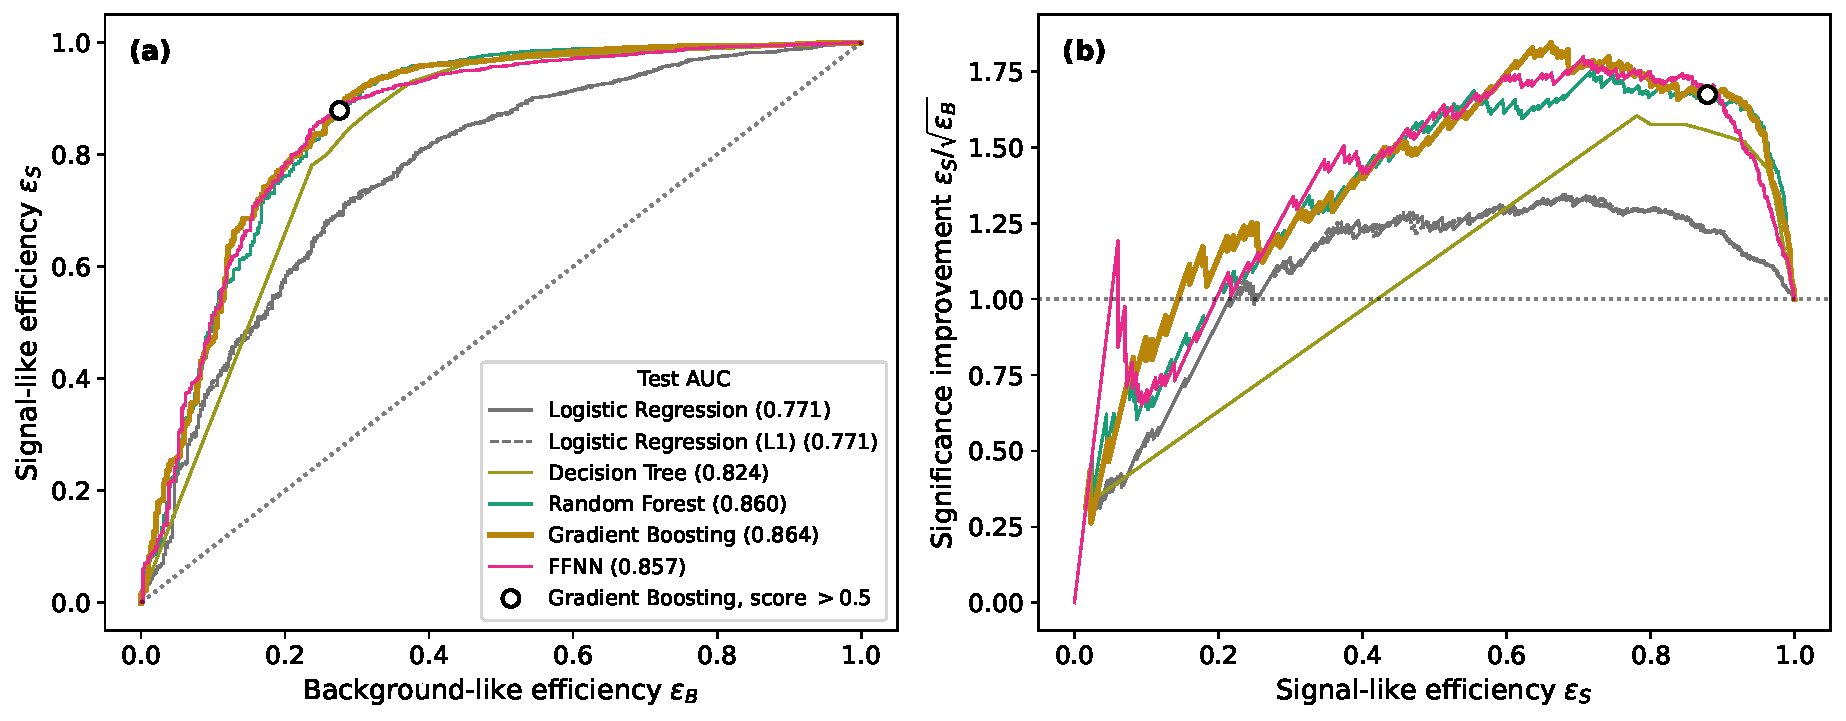
\includegraphics[width=0.95\textwidth]{figures/ml_nominal_roc.pdf}
\caption{Test-set performance of the classifiers: (a) ROC curves, with the test AUC of each model in the legend (Table~\ref{tab:ml_models}); (b) significance improvement $\varepsilon_S/\sqrt{\varepsilon_B}$ of a cut on the score as a function of the signal-like efficiency, where $1$ is no selection and $\varepsilon_{S,B}$ are the fractions of signal-like and background-like candidates kept. The reference model is drawn thicker, and the two logistic regressions overlap. The circle marks the cut on the reference score used in Appendix~\ref{sec:ml_stability}.}
\label{fig:ml_roc}
\end{figure*}
\begin{figure*}[!t]
\centering
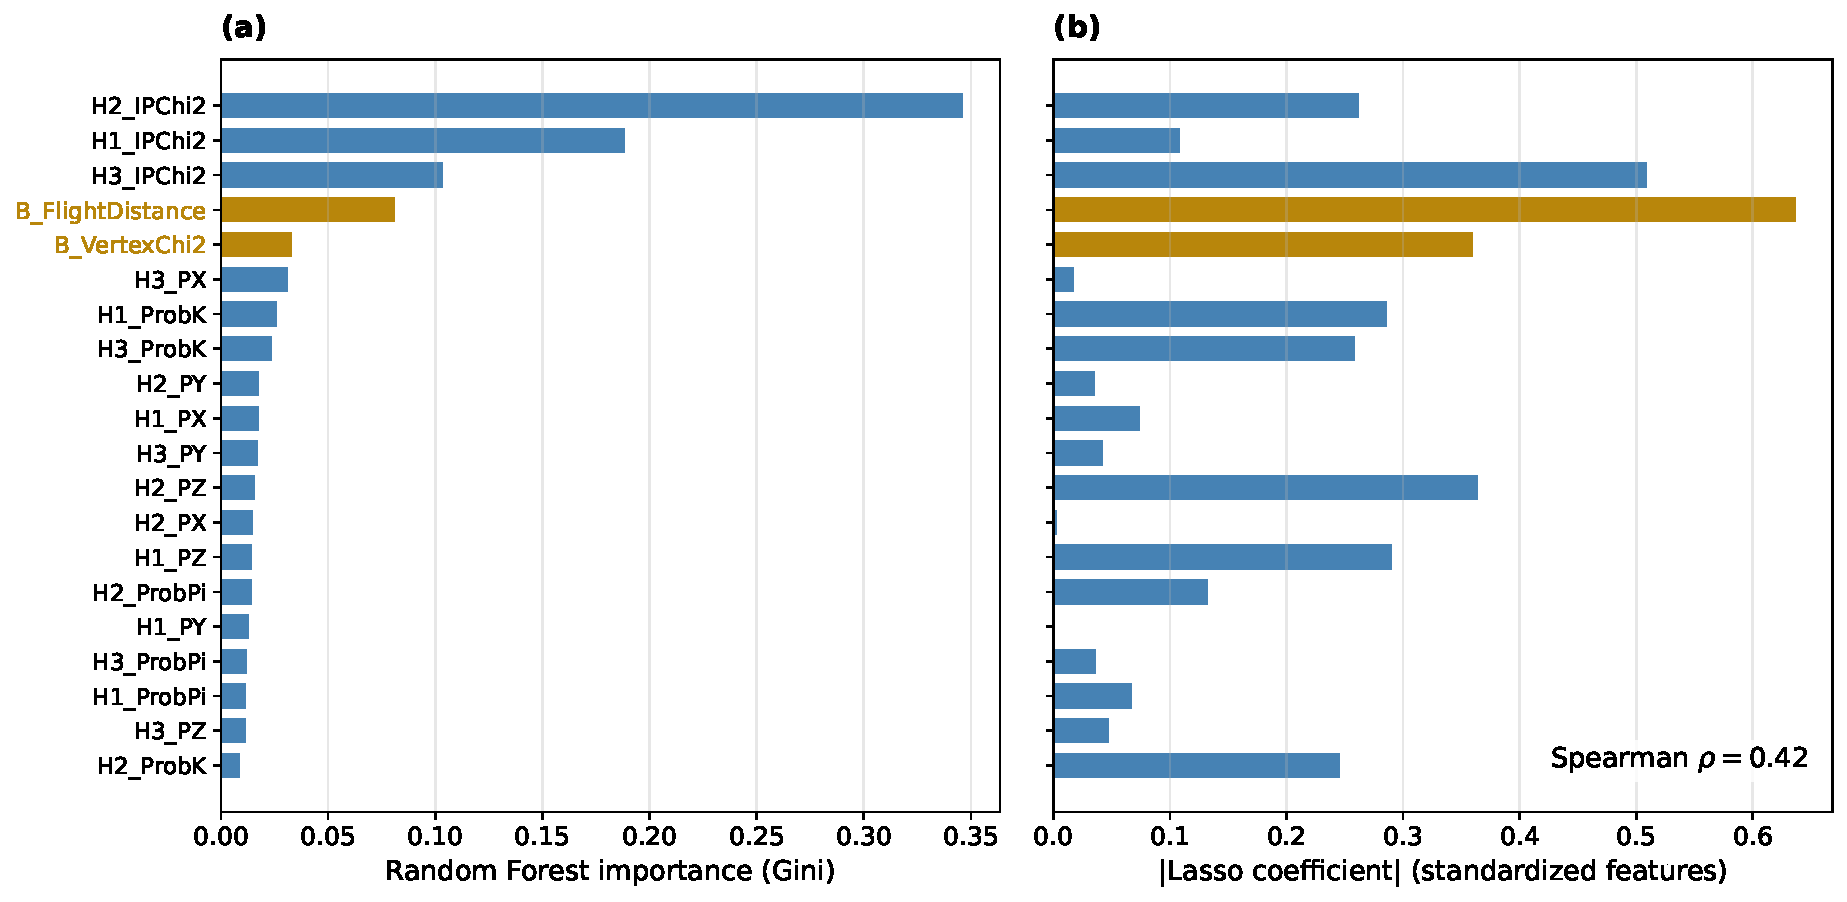
\includegraphics[width=0.95\textwidth]{figures/ml_nominal_features.pdf}
\caption{Random Forest feature importance (Gini, a) and magnitude of the Lasso coefficient of the standardized feature (b) for the 20 features, both ordered by Random Forest importance; the two $B$-candidate variables are highlighted.}
\label{fig:ml_features}
\end{figure*}
\begin{figure*}[!t]
\centering
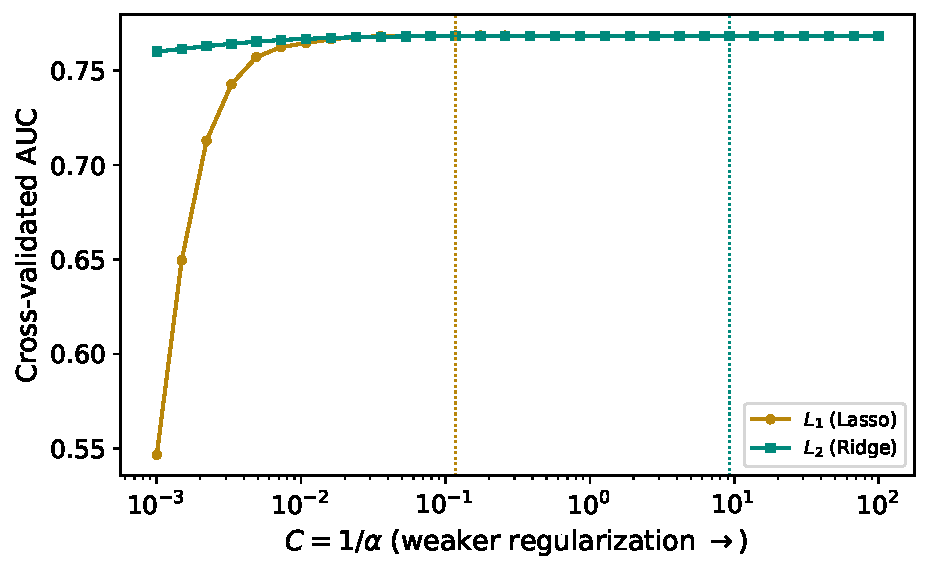
\includegraphics[width=0.5\textwidth]{figures/ml_regularization.pdf}
\caption{Cross-validated AUC of the logistic regression against the inverse regularization strength $C=1/\alpha$ ($30$ log-spaced values), for the $L_1$ (Lasso) and $L_2$ (Ridge) penalties; the dotted lines mark the optimum of each.}
\label{fig:ml_regularization}
\end{figure*}
\begin{figure*}[!t]
\centering
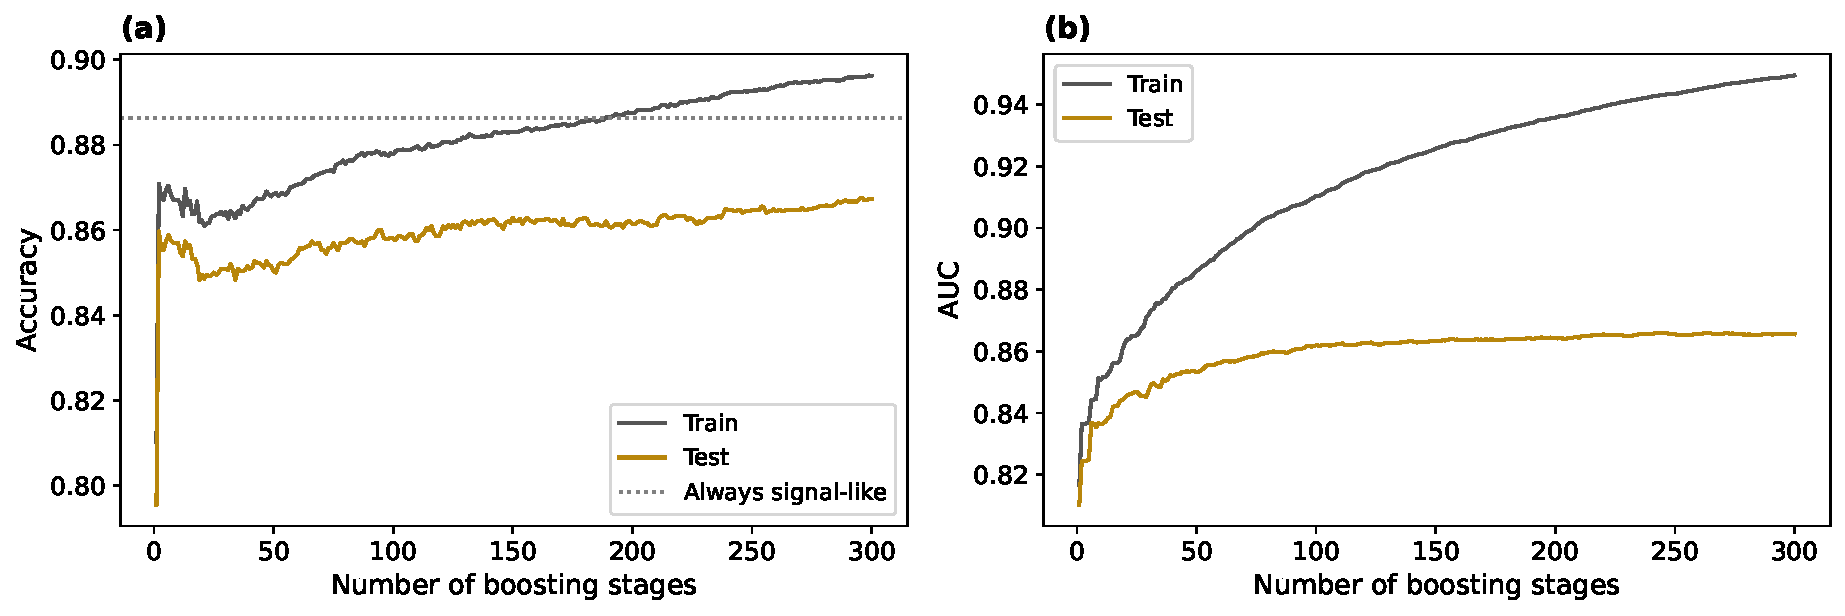
\includegraphics[width=0.95\textwidth]{figures/ml_nominal_bias_variance.pdf}
\caption{Gradient boosting: (a) accuracy at the $0.5$ threshold and (b) AUC on the training and test sets as a function of the number of boosting stages. The dotted line is the accuracy of always predicting the signal-like class.}
\label{fig:ml_bias_variance}
\end{figure*}
\begin{figure*}[!t]
\centering
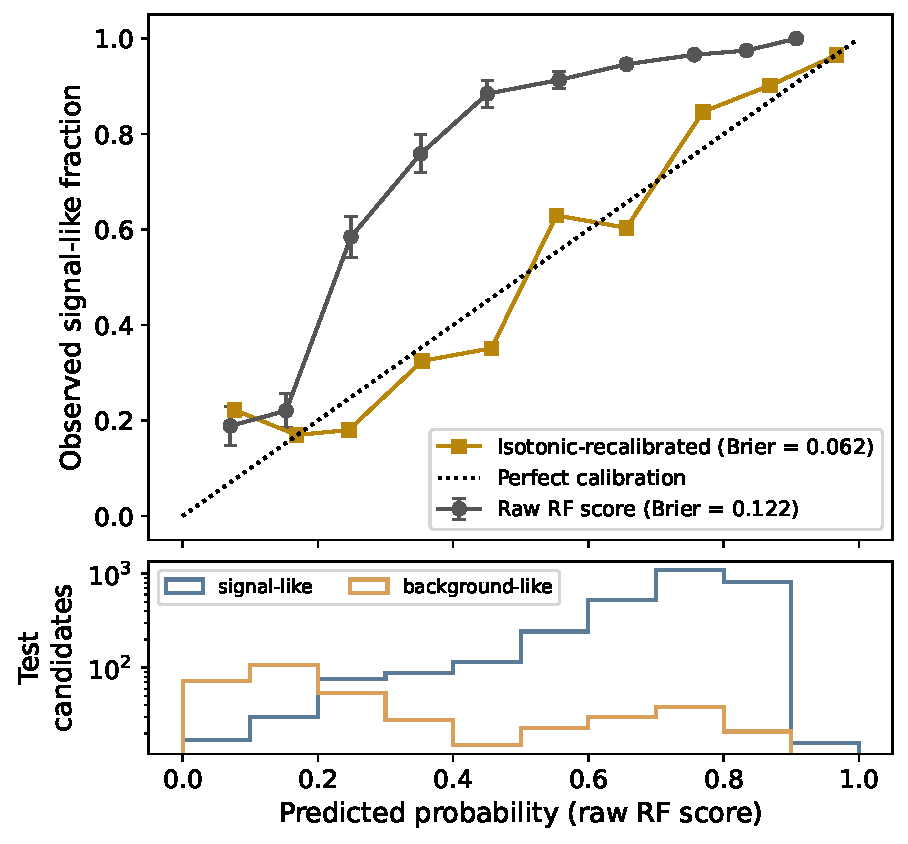
\includegraphics[width=0.5\textwidth]{figures/ml_nominal_calibration.pdf}
\caption{Reliability diagram of the Random Forest on the test set: observed fraction of signal-like candidates vs.\ predicted probability, for the raw score (with binomial uncertainties) and for the isotonic-recalibrated one. Bottom: distribution of the raw score for the two weak-label classes; the low-probability bins contain few candidates.}
\label{fig:ml_calibration}
\end{figure*}
\begin{figure*}[!t]
\centering
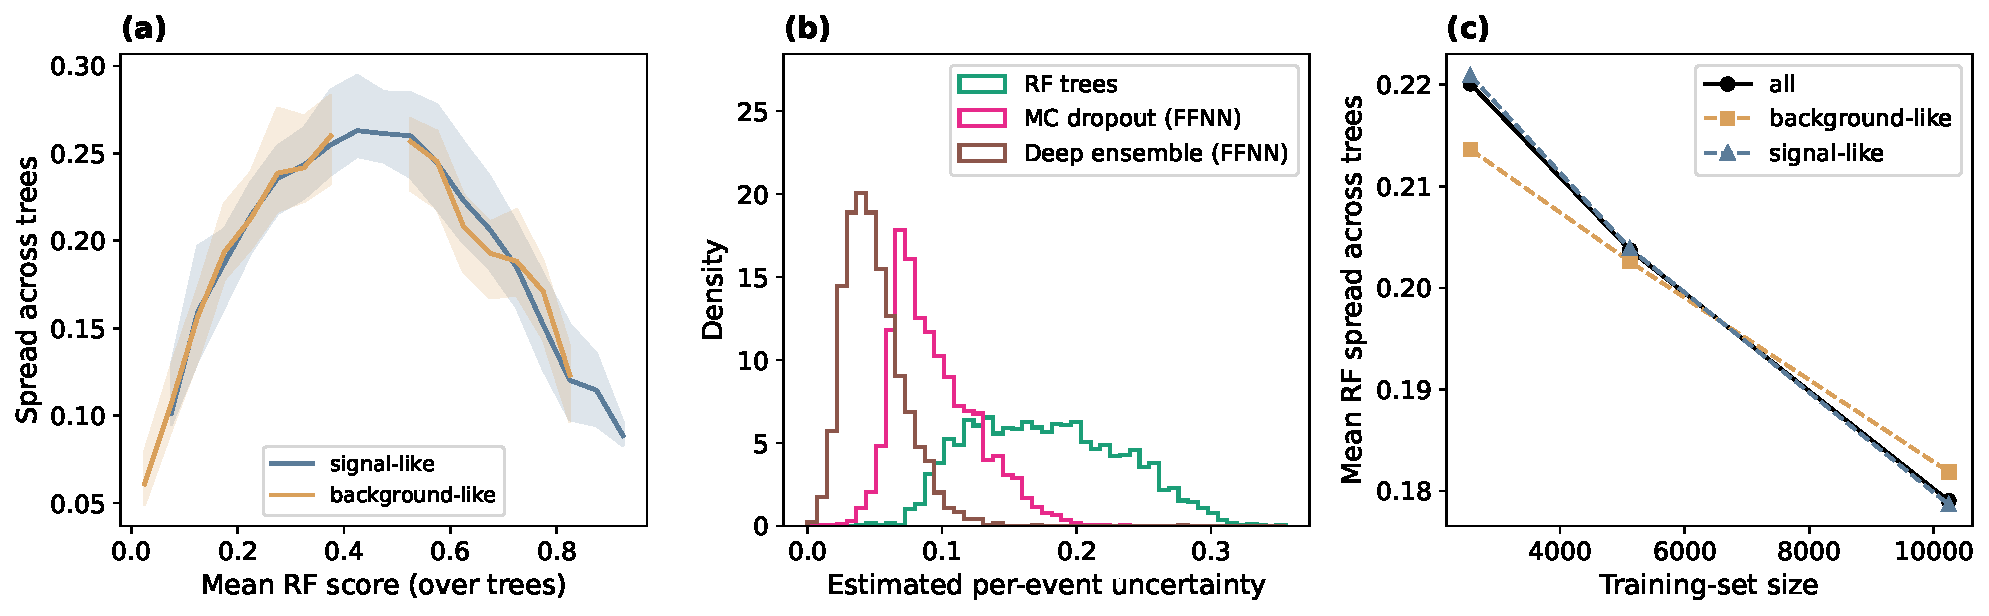
\includegraphics[width=0.95\textwidth]{figures/ml_nominal_uncertainty.pdf}
\caption{(a) Spread across the Random Forest trees vs.\ mean tree score, median and 16--84\% band of the test candidates of each weak-label class. (b) Distributions of the per-candidate uncertainty from the Random Forest trees, MC dropout and the deep ensemble. (c) Mean Random Forest spread vs.\ training-set size, for all, background-like and signal-like test candidates.}
\label{fig:ml_uncertainty}
\end{figure*}
\begin{figure*}[!t]
\centering
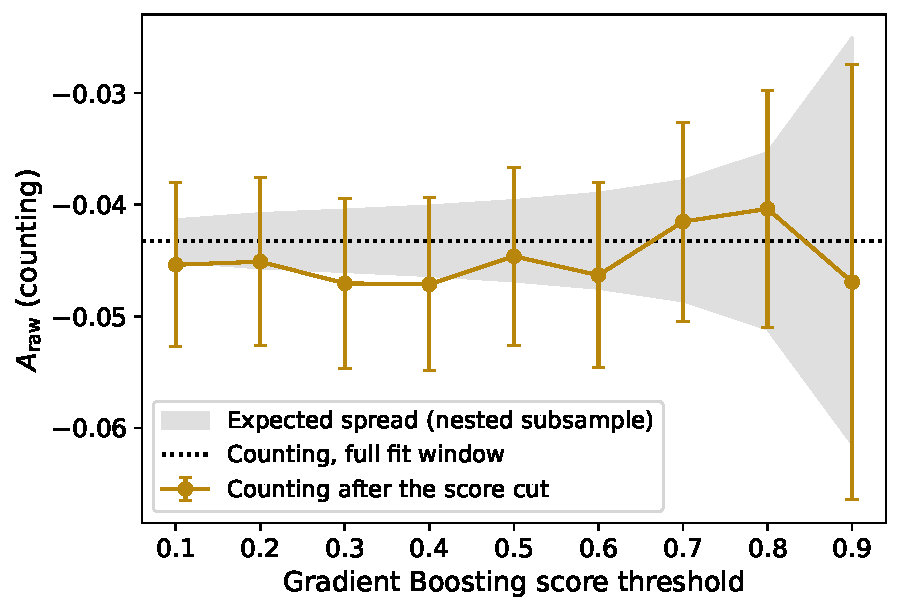
\includegraphics[width=0.5\textwidth]{figures/ml_nominal_threshold.pdf}
\caption{Counting asymmetry after a cut on the gradient-boosting score, vs.\ threshold, with its binomial uncertainty. Dotted line: counting asymmetry of the full fit window; band: expected statistical spread of a nested subsample around it, $\pm\sqrt{\sigma_{\mathrm{sub}}^2-\sigma_{\mathrm{full}}^2}$.}
\label{fig:ml_threshold}
\end{figure*}
\begin{figure*}[!t]
\makeatletter\def\@captype{table}\makeatother
\centering
\begin{tabular}{lccccc}
\toprule
Method & Full sample & Score $>0.5$ & Shift (expected) & Score $>0.73$ & Shift (expected) \\
\midrule
Bayesian fit    & $-0.0443\pm0.0085$ & $-0.0451\pm0.0087$ & $-0.0008\,(0.0018)$ & $-0.0404\pm0.0097$ & $+0.0039\,(0.0047)$ \\
Frequentist fit & $-0.0441\pm0.0085$ & $-0.0447\pm0.0086$ & $-0.0006\,(0.0012)$ & $-0.0401\pm0.0097$ & $+0.0040\,(0.0048)$ \\
Counting        & $-0.0432\pm0.0071$ & $-0.0446\pm0.0080$ & $-0.0014\,(0.0036)$ & $-0.0381\pm0.0093$ & $+0.0051\,(0.0059)$ \\
\bottomrule
\end{tabular}
\caption{$\Araw$ on the full fit window ($19{,}731$ candidates) and after the cuts on the gradient-boosting score at $0.5$ ($15{,}709$ candidates) and at $0.73$ ($11{,}658$), the maximum of the significance improvement of Fig.~\ref{fig:ml_roc}, by the three methods. The expected shift is the statistical spread of a nested subsample, $\sqrt{\sigma_{\mathrm{sub}}^2-\sigma_{\mathrm{full}}^2}$. Counting includes the background.}
\label{tab:three_methods}
\end{figure*}
\begin{figure*}[!t]
\centering
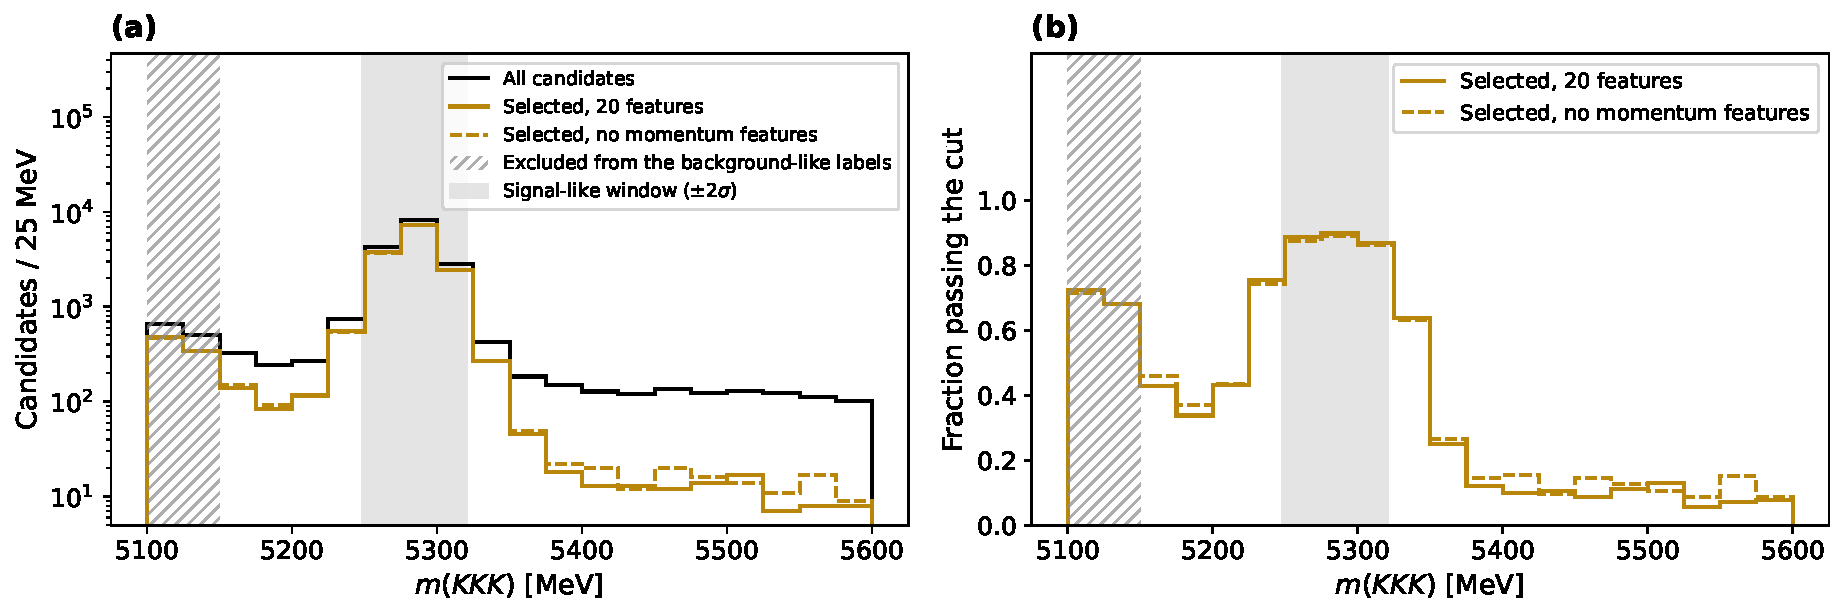
\includegraphics[width=0.95\textwidth]{figures/ml_nominal_mass_after_cut.pdf}
\caption{(a) Mass spectrum of all candidates and of those with gradient-boosting score $>0.5$, for the 20-feature classifier and for one trained without the kaon momentum components (25\,MeV bins). (b) Fraction of candidates passing the cut. Hatched: the region below $5150\,\MeV$ excluded from the background-like labels; grey: the signal-like window.}
\label{fig:ml_mass_cut}
\end{figure*}
\begin{figure*}[!t]
\centering
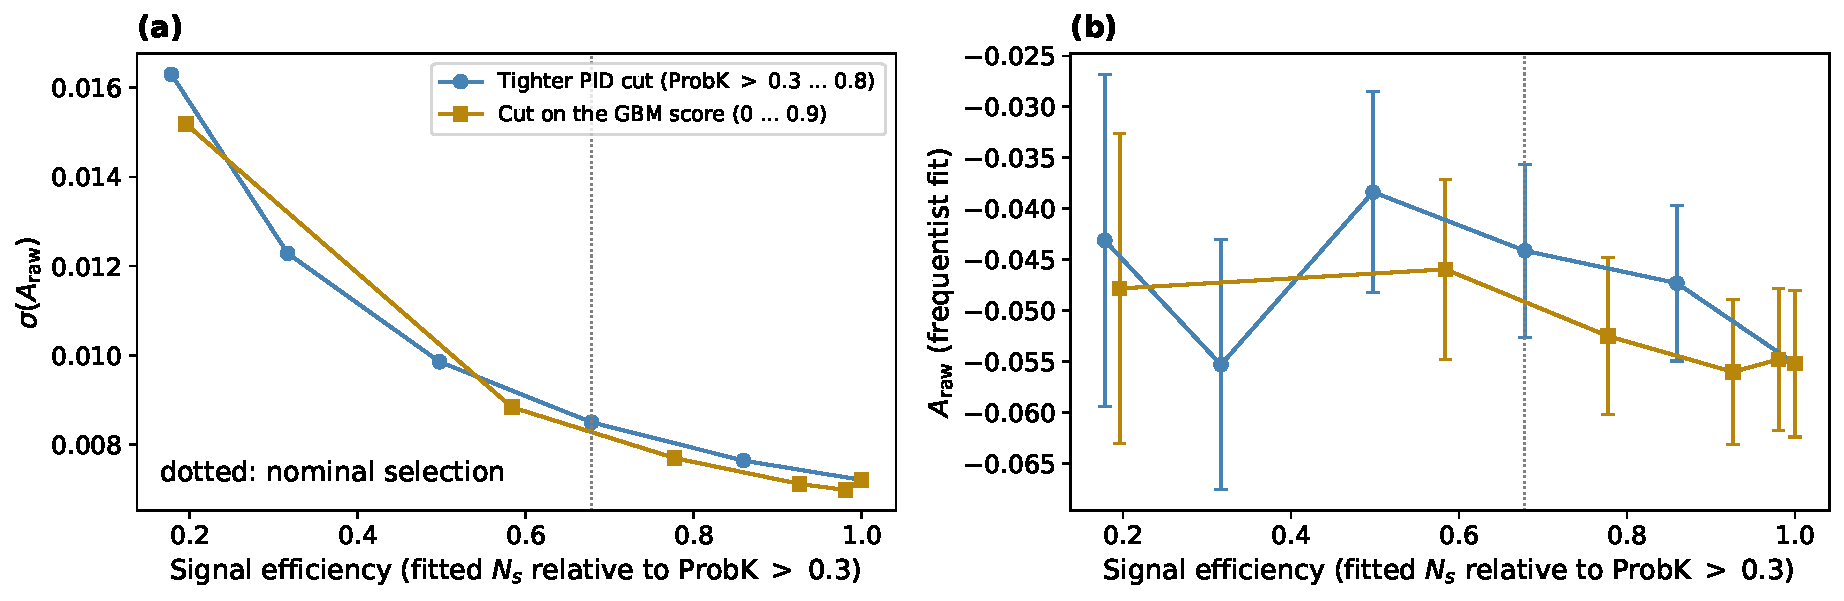
\includegraphics[width=0.95\textwidth]{figures/ml_nominal_high_background.pdf}
\caption{High-background sample ($\texttt{ProbK}>0.3$): (a) statistical uncertainty and (b) value of $\Araw$ from the frequentist fit vs signal efficiency, for tighter identification cuts ($\texttt{ProbK}>0.3,\dots,0.8$) and for cuts on the score of the classifier retrained on this sample ($0,\dots,0.9$). The dotted line marks the nominal selection ($\texttt{ProbK}>0.5$). The samples are nested, so their uncertainties are correlated.}
\label{fig:ml_high_bkg}
\end{figure*}
\begin{figure*}[!t]
\centering
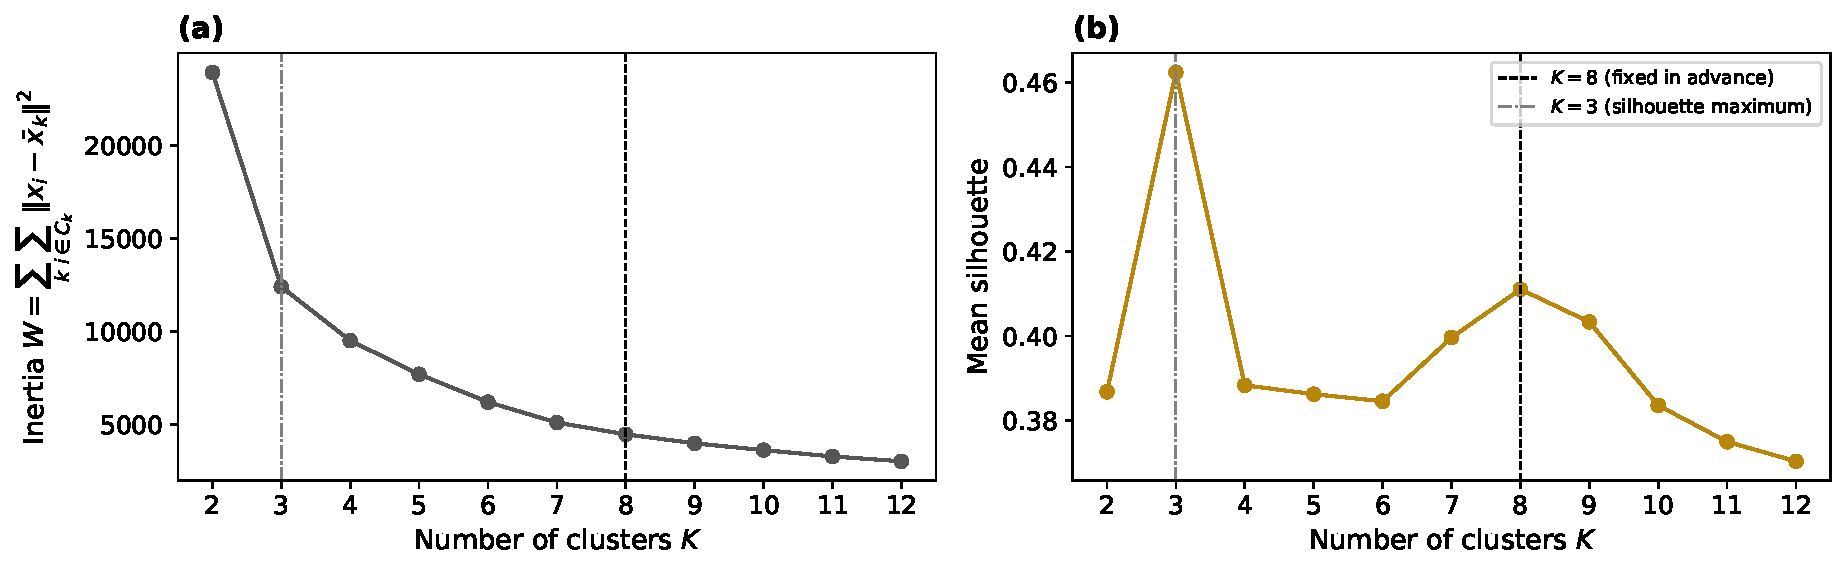
\includegraphics[width=0.85\textwidth]{figures/ml_kmeans_selection.pdf}
\caption{(a) Inertia and (b) mean silhouette of the $K$-means partition of the Dalitz plane for $K=2$--$12$; the dashed line marks the $K=8$ fixed in advance and the dash-dotted line the maximum of the silhouette, $K=3$.}
\label{fig:ml_kmeans_sel}
\end{figure*}
\begin{figure*}[!t]
\centering
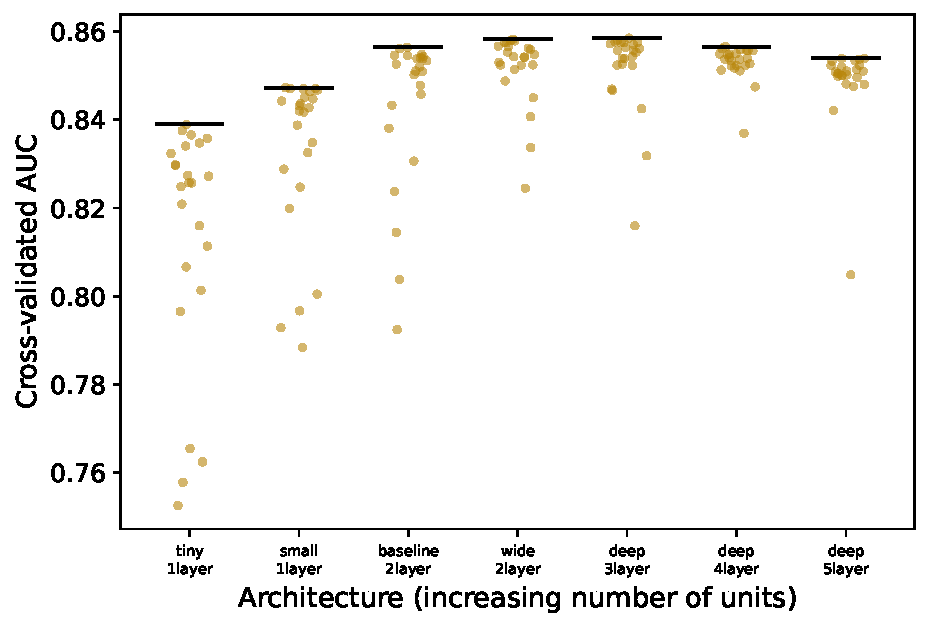
\includegraphics[width=0.5\textwidth]{figures/ml_ffnn_search.pdf}
\caption{Cross-validated AUC of the $168$ FFNN configurations (dots) for each of the seven architectures, ordered by number of units; the black segment marks the best configuration of each architecture.}
\label{fig:ml_ffnn_search}
\end{figure*}
\begin{figure*}[!t]
\makeatletter\def\@captype{table}\makeatother
\centering
\begin{tabular}{lllc}
\toprule
Model & \pcell{7cm}{Grid} & Best configuration & CV AUC / Test AUC (default) \\
\midrule
Random Forest & \pcell{7cm}{\texttt{n\_estimators} $200$--$1200$, \texttt{max\_depth} $6$--$12$ or none, \texttt{min\_samples\_leaf} $5$--$40$} & $400$, $12$, $5$ & $0.8706$ / $0.8656$ ($0.8604$) \\
Gradient Boosting & \pcell{7cm}{\texttt{n\_estimators} $100$--$500$, \texttt{max\_depth} $1$--$5$, \texttt{learning\_rate} $0.01$--$0.1$} & $300$, $2$, $0.1$ & $0.8684$ / $0.8650$ ($0.8643$) \\
\bottomrule
\end{tabular}
\caption{Hyperparameter search for the tree ensembles ($120$ and $100$ configurations, 5-fold cross-validation repeated 10 times, balanced class weights). The test AUC of the best configuration is compared with that of the default of Table~\ref{tab:ml_models} (in parentheses); the bootstrap uncertainty of each test AUC is $0.012$.}
\label{tab:ml_hyperparams}
\end{figure*}
\begin{figure*}[!t]
\makeatletter\def\@captype{table}\makeatother
\centering
\begin{tabular}{llccc}
\toprule
Architecture & Layers & Dropout & Learning rate & CV AUC \\
\midrule
\texttt{deep\_3layer} (best) & $[64,32,16]$ & $0.2$ & $0.003$ & $0.8585\pm0.0174$ \\
\texttt{wide\_2layer}        & $[64,32]$    & $0.3$ & $0.003$ & $0.8582\pm0.0175$ \\
\texttt{deep\_3layer}        & $[64,32,16]$ & $0.3$ & $0.003$ & $0.8580\pm0.0187$ \\
\texttt{wide\_2layer}        & $[64,32]$    & $0.3$ & $0.005$ & $0.8579\pm0.0184$ \\
\texttt{wide\_2layer}        & $[64,32]$    & $0.4$ & $0.005$ & $0.8579\pm0.0187$ \\
\bottomrule
\end{tabular}
\caption{Top five of the $168$ FFNN configurations ($7$ architectures from one hidden layer of 8 units to five layers $[128,64,32,16,8]$, dropout $0.1$--$0.4$, learning rates $0.0002$--$0.005$; 5-fold cross-validation repeated twice). The five are within $0.0007$ of each other, far below the fold-to-fold spread: the optimum is a plateau. The best configuration has test AUC $0.8606$, against $0.8568$ for the default architecture ($\pm0.005$ over initializations).}
\label{tab:ml_ffnn_search}
\end{figure*}

\FloatBarrier

\section{Local Asymmetry in the Dalitz Plane}
\label{app:ext_dalitz}
\emph{In short: the homogeneity test in other samples and in the two magnet polarities, the permutation test and the $\phi(1020)$ band.}
\subsection{Homogeneity Test: Signal Window, Vetoes, Grids and Magnet Split}
\label{app:dalitz_homog}
\emph{In short: the homogeneity test holds in the signal window, with the charm vetoes and for other grids, and the structure is the same in the two magnet polarities ($\chi^2=23.0$ for $29$ bins).}

\subsection{Distribution of the Homogeneity Statistic under Charge Permutation}
\label{app:dalitz_perm}
\emph{In short: shuffling the charges reproduces the $\chi^2$ distribution of a uniform asymmetry, and the observed value lies far beyond all $2000$ permutations (Fig.~\ref{fig:dalitz_perm}).}

Figure~\ref{fig:dalitz_perm} shows the homogeneity statistic $\chi^2=\sum_iS_i^2$ of the $8\times8$ grid for $2000$ random permutations of the charges, the $\chi^2$ distribution with $31$ degrees of freedom and the observed value.

\begin{figure*}[!t]
\centering
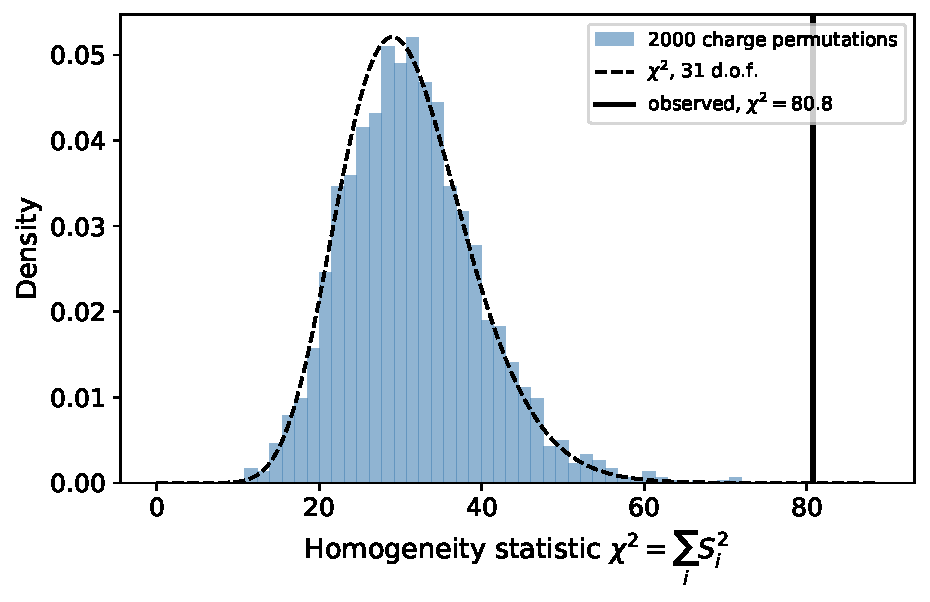
\includegraphics[width=0.5\textwidth]{figures/dalitz_permutation.pdf}
\caption{Homogeneity statistic $\chi^2=\sum_iS_i^2$ of the $8\times8$ Dalitz grid for $2000$ random permutations of the charges (histogram), $\chi^2$ distribution with $31$ degrees of freedom (dashed) and observed value (line).}
\label{fig:dalitz_perm}
\end{figure*}

\subsection{Asymmetry in the $\phi(1020)$ Band and in the Significant Bins}
\label{app:dalitz_phi}
\emph{In short: the band of the $\phi(1020)$ has no asymmetry, the negative asymmetry is outside it and larger when the $\phi$ candidates are removed (Fig.~\ref{fig:dalitz_phi}b); in the region of the published analysis the $B^-$ peak is visibly smaller (Fig.~\ref{fig:dalitz_region}b).}

Figure~\ref{fig:dalitz_phi} shows (a) the distribution of $m_{\mathrm{lo}}(K^+K^-)$ around the $\phi(1020)$ with the band used, and (b) the counting asymmetry of all candidates, of the $\phi$ band, of the region outside it and of the two significant bins with and without the $\phi$ candidates.

\begin{figure*}[!t]
\centering
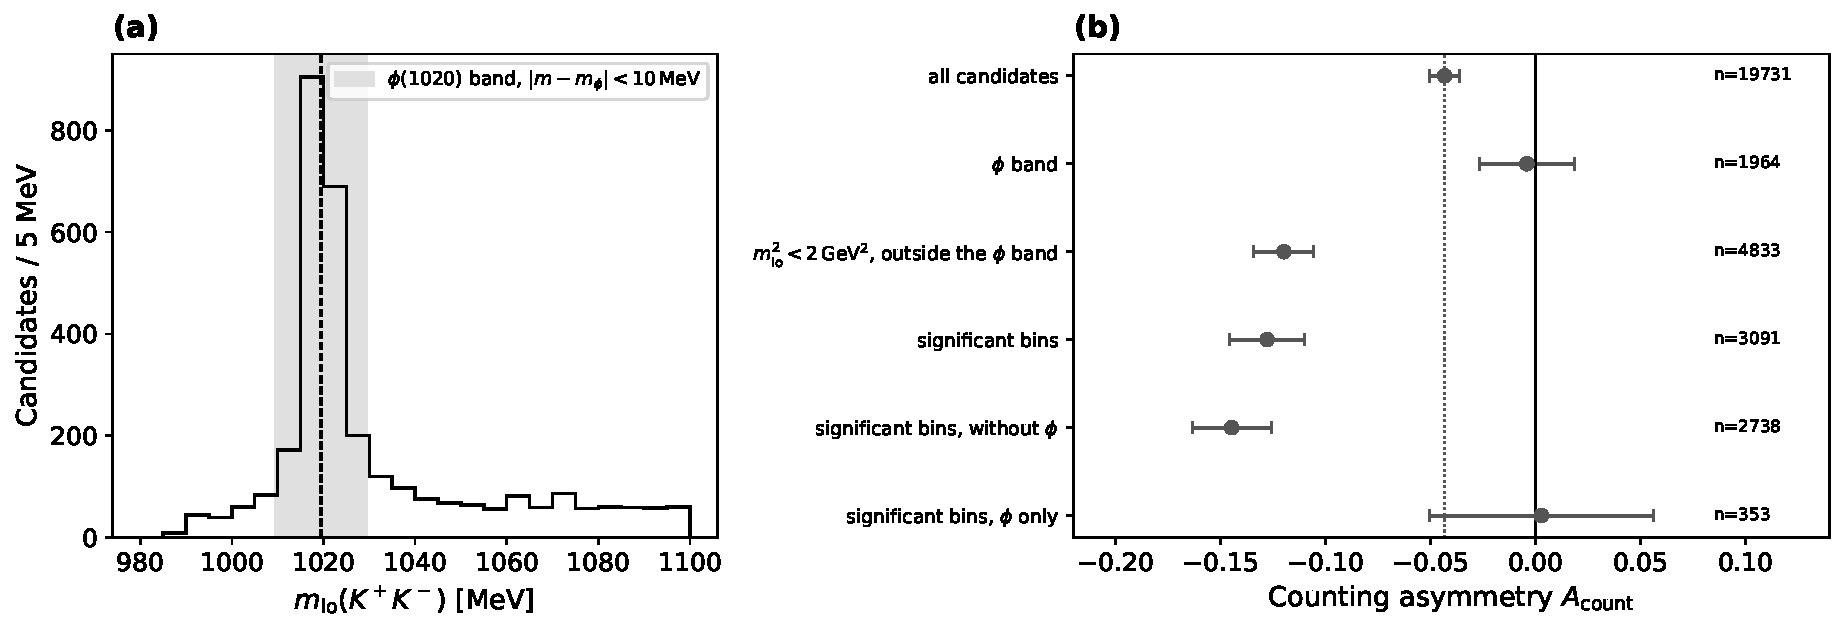
\includegraphics[width=0.9\textwidth]{figures/dalitz_phi_band.pdf}
\caption{(a) Distribution of $m_{\mathrm{lo}}(K^+K^-)$ around the $\phi(1020)$ ($5\,\MeV$ bins) and band used (shaded). (b) Counting asymmetry, with binomial uncertainty and number of candidates, of all candidates (dotted line), of the $\phi$ band, of the region $m^2_{\mathrm{lo}}<2\,\GeV^2$ outside the band, and of the two significant bins of Fig.~\ref{fig:bayes_dalitz}, with and without the candidates of the $\phi$ band, and of those candidates alone.}
\label{fig:dalitz_phi}
\end{figure*}

Figure~\ref{fig:dalitz_region} shows (a) the ordered Dalitz plot with the squared masses of the $\phi(1020)$, $D^0$, $J/\psi$ and $\chi_{c0}$ and the region of the published analysis, and (b) the mass spectra of $B^+$ and $B^-$ candidates in that region.

\begin{figure*}[!t]
\centering
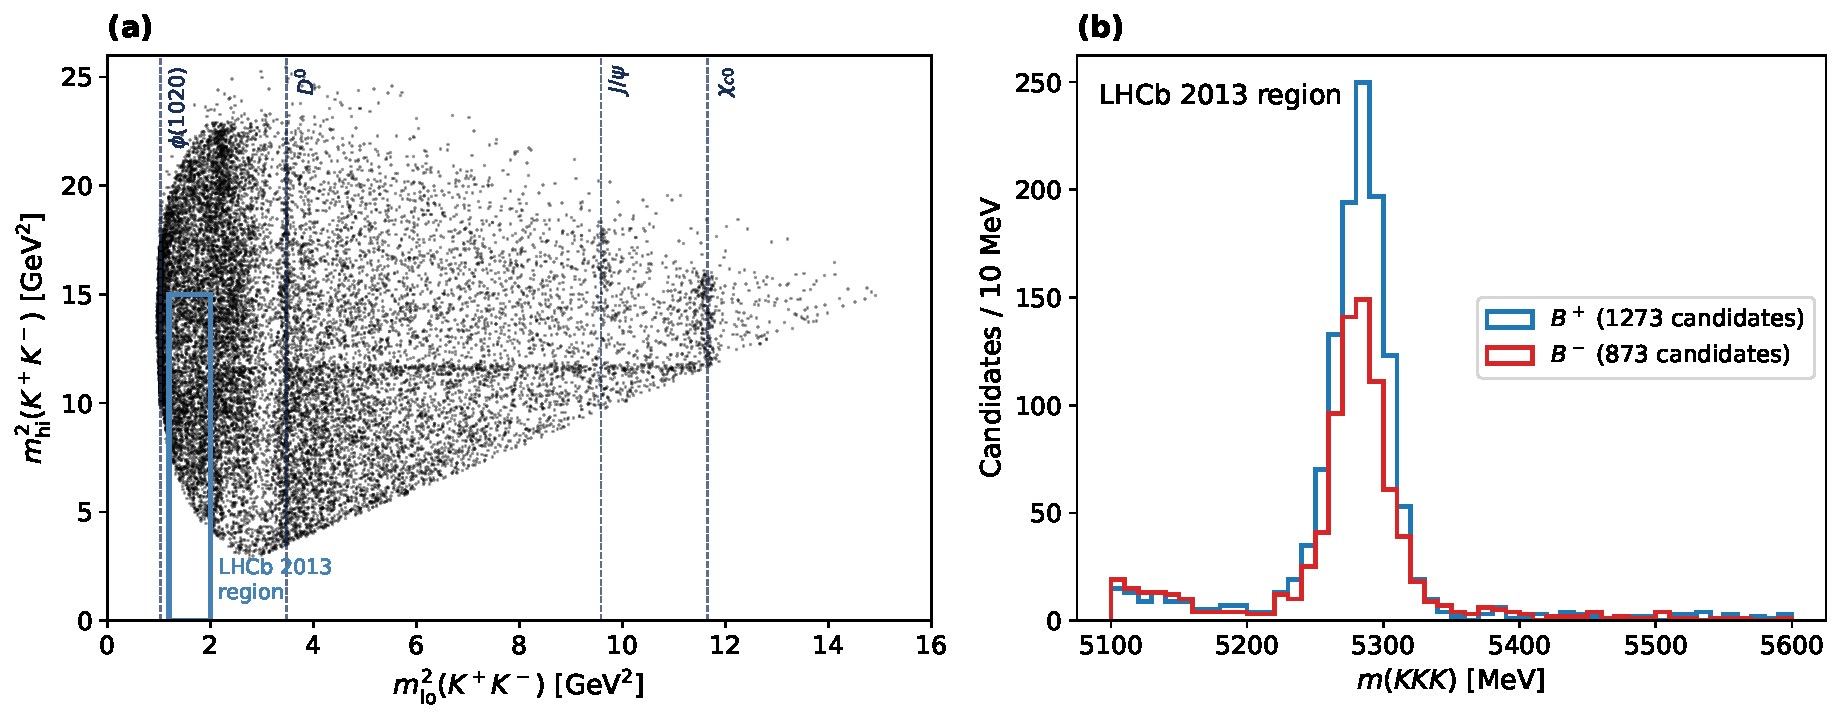
\includegraphics[width=0.80\textwidth]{figures/ml_nominal_dalitz_region.pdf}
\caption{(a) Ordered Dalitz plot of the candidates in the fit window, with the squared masses of the $\phi(1020)$, $D^0$, $J/\psi$ and $\chi_{c0}$ (dashed) and the region of the published analysis of the same data~\cite{lhcb_cpv_2013} (box). (b) Mass spectra of $B^+$ and $B^-$ candidates in that region, same binning: the $B^-$ peak is visibly smaller.}
\label{fig:dalitz_region}
\end{figure*}

\section{Systematic Uncertainties}
\label{app:syst}
\emph{In short: every fit of the nominal model and of its variants with both methods, the validation of the combination rule on nested samples and the stability scans of the frequentist fit.}
\subsection{All Fits of the Nominal Model and of Its Variants}
\label{sec:syst_tables}
\emph{In short: the Bayesian and frequentist results of every variant and cross-check side by side (Table~\ref{tab:bayes_all}), and the shift of each variant with its expected spread $\sigma_B$ (Table~\ref{tab:syst}).}

Table~\ref{tab:bayes_all} lists, for every variant, the number of candidates, the Bayesian median and $68\%$ credible interval of $\Araw$, the binned goodness of fit and the frequentist estimate with its Hesse uncertainty.

\begin{figure*}[!t]
\makeatletter\def\@captype{table}\makeatother
\centering
\begin{tabular}{lrccc|c}
\toprule
Fit & $n$ & $\Araw$ Bayesian (median) & 68\% CI & $\chi^2$/ndof & $\Araw$ frequentist \\
\midrule
Nominal & $19731$ & $-0.0443$ & $[-0.0528,-0.0358]$ & $164.1/88$ & $-0.0441\pm0.0085$ \\
\multicolumn{6}{l}{\emph{Systematic variants (Sec.~\ref{sec:syst})}} \\
Window $[5050,5600]$ & $21164$ & $-0.0446$ & $[-0.0531,-0.0362]$ & $217.4/98$ & $-0.0445\pm0.0085$ \\
Window $[5150,5600]$ & $18566$ & $-0.0444$ & $[-0.0528,-0.0359]$ & $141.5/78$ & $-0.0446\pm0.0088$$^\dagger$ \\
Window $[5100,5450]$ & $19004$ & $-0.0440$ & $[-0.0524,-0.0357]$ & $136.9/58$ & $-0.0442\pm0.0085$ \\
Window $[5100,5700]$ & $20191$ & $-0.0456$ & $[-0.0540,-0.0373]$ & $200.2/108$ & $-0.0455\pm0.0085$ \\
Single exponential & $19731$ & $-0.0480$ & $[-0.0564,-0.0395]$ & $297.7/92$ & $-0.0481\pm0.0085$ \\
Background shape shared & $19731$ & $-0.0480$ & $[-0.0564,-0.0397]$ & $174.1/91$ & $-0.0481\pm0.0083$ \\
Symmetric background & $19731$ & $-0.0471$ & $[-0.0552,-0.0388]$ & $169.8/89$ & $-0.0472\pm0.0084$ \\
Crystal Ball signal & $19731$ & $-0.0445$ & $[-0.0529,-0.0363]$ & $131.0/86$ & $-0.0447\pm0.0085$ \\
$\mu,\sigma$ per charge & $19731$ & $-0.0443$ & $[-0.0527,-0.0356]$ & $164.2/86$ & $-0.0442\pm0.0087$ \\
$\texttt{ProbK}>0.4$ & $26553$ & $-0.0474$ & $[-0.0550,-0.0399]$ & $175.6/88$ & $-0.0473\pm0.0076$ \\
$\texttt{ProbK}>0.6$ & $13981$ & $-0.0385$ & $[-0.0482,-0.0289]$ & $145.0/88$ & $-0.0384\pm0.0099$ \\
$\texttt{ProbPi}<0.4$ & $17984$ & $-0.0421$ & $[-0.0506,-0.0333]$ & $150.1/88$ & $-0.0421\pm0.0088$ \\
$\texttt{ProbPi}<0.6$ & $20953$ & $-0.0446$ & $[-0.0529,-0.0366]$ & $159.0/88$ & $-0.0448\pm0.0083$ \\
\multicolumn{6}{l}{\emph{Cross-checks (Secs.~\ref{sec:bayes_mcmc}, \ref{sec:bayes_checks})}} \\
Dispersed start, run 1 & $19731$ & $-0.0446$ & $[-0.0529,-0.0360]$ & $164.1/88$ & -- \\
Dispersed start, run 2 & $19731$ & $-0.0442$ & $[-0.0528,-0.0356]$ & $164.1/88$ & -- \\
Magnet down & $11636$ & $-0.0497$ & $[-0.0607,-0.0386]$ & $153.1/88$ & -- \\
Magnet up & $8095$ & $-0.0378$ & $[-0.0507,-0.0251]$ & $150.3/88$ & -- \\
Narrow prior, $A\in(-0.3,0.3)$ & $19731$ & $-0.0443$ & $[-0.0528,-0.0358]$ & $164.1/88$ & -- \\
$D^0$ veto & $18744$ & $-0.0496$ & $[-0.0584,-0.0409]$ & $159.1/88$ & $-0.0493\pm0.0087$ \\
$D^0$, $J/\psi$, $\chi_{c0}$ vetoes & $16367$ & $-0.0423$ & $[-0.0516,-0.0329]$ & $140.1/88$ & $-0.0421\pm0.0094$ \\
\bottomrule
\end{tabular}
\caption{All fits of the nominal model and of its variants: number of candidates, Bayesian posterior median and 68\% credible interval of $\Araw$, binned goodness of fit ($10\,\MeV$ bins), and frequentist estimate with its Hesse uncertainty (Sec.~\ref{sec:frequentist}; fitted on the same candidates; the cross-checks of the Bayesian fits that have no frequentist counterpart in this work are marked --). $^\dagger$ Uncertainty scaled from the number of events, since the Hesse matrix of that fit is not accurate. Every fit uses 32 walkers and $25{,}000$ steps.}
\label{tab:bayes_all}
\end{figure*}

Table~\ref{tab:syst} gives the shift of each variant, the expected spread $\sigma_B$ for the variants that change the sample, and the uncertainty of each group.

\begin{figure*}[!t]
\makeatletter\def\@captype{table}\makeatother
\centering
\small
\resizebox{\ifdim\width>\linewidth\linewidth\else\width\fi}{!}{\begin{tabular}{llcc}
\toprule
Group & Variant & Bayesian & Frequentist \\
\midrule
Window & $[5050,5600]$ & $-0.0003$ ($0.0009$) & $-0.0004$ ($0.0005$) \\
 & $[5150,5600]$ & $-0.0001$ ($0.0007$) & $-0.0005$ ($0.0021$) \\
 & $[5100,5450]$ & $+0.0002$ ($0.0009$) & $-0.0001$ ($0.0003$) \\
 & $[5100,5700]$ & $-0.0014$ ($0.0010$) & $-0.0014$ ($0.0001$) \\
& \emph{group uncertainty} & $\mathit{0.0014}$ & $\mathit{0.0014}$ \\
\midrule
Background & single exponential (rejected) & $-0.0037$ & $-0.0039$ \\
 & shape shared between charges & $-0.0037$ & $-0.0040$ \\
 & symmetric, $A_b=0$ & $-0.0028$ & $-0.0031$ \\
& \emph{group uncertainty} & $\mathit{0.0037}$ & $\mathit{0.0040}$ \\
\midrule
Signal & Crystal Ball & $-0.0002$ & $-0.0006$ \\
 & $\mu,\sigma$ per charge & $-0.0000$ & $-0.0001$ \\
& \emph{group uncertainty} & $\mathit{0.0002}$ & $\mathit{0.0006}$ \\
\midrule
Preselection & $\texttt{ProbK}>0.4$ & $-0.0032$ ($0.0038$) & $-0.0032$ ($0.0037$) \\
 & $\texttt{ProbK}>0.6$ & $+0.0058$ ($0.0048$) & $+0.0058$ ($0.0050$) \\
 & $\texttt{ProbPi}<0.4$ & $+0.0022$ ($0.0022$) & $+0.0020$ ($0.0023$) \\
 & $\texttt{ProbPi}<0.6$ & $-0.0004$ ($0.0020$) & $-0.0006$ ($0.0017$) \\
& \emph{group uncertainty} & $\mathit{0.0058}$ & $\mathit{0.0058}$ \\
\midrule
\multicolumn{2}{l}{Total (quadrature)} & $0.0070$ & $0.0072$ \\
\bottomrule
\end{tabular}}
\caption{Systematic study common to the Bayesian and frequentist fits: shift $\Delta$ of $\Araw$ for each variant and, in parentheses and for the variants that change the sample, the expected statistical spread $\sigma_B$ of the shift. The largest contributing shift of each group is its uncertainty (italics); the groups are added in quadrature. The single exponential is rejected by the data and excluded. For the window $[5150,5600]$ the frequentist uncertainty is scaled from the number of events, since the Hesse matrix of that fit is not accurate.}
\label{tab:syst}
\end{figure*}

\subsection{Validation of the Rule for Nested Samples}
\label{sec:checks_barlow}
\emph{In short: the spread of the shift of $\hat A$ between a sample and its tighter-identification subsample is the one given by the quadrature difference of the uncertainties (Fig.~\ref{fig:checks_barlow}).}

Figure~\ref{fig:checks_barlow} shows the shift of $\hat A$ between the nominal sample and a tighter selection, divided by the median $\sigma_B$, in $300$ bootstrap replicas, for (a) $\texttt{ProbK}>0.6$ and (b) $\texttt{ProbPi}<0.4$, with a standard normal distribution.

\begin{figure*}[!t]
\centering
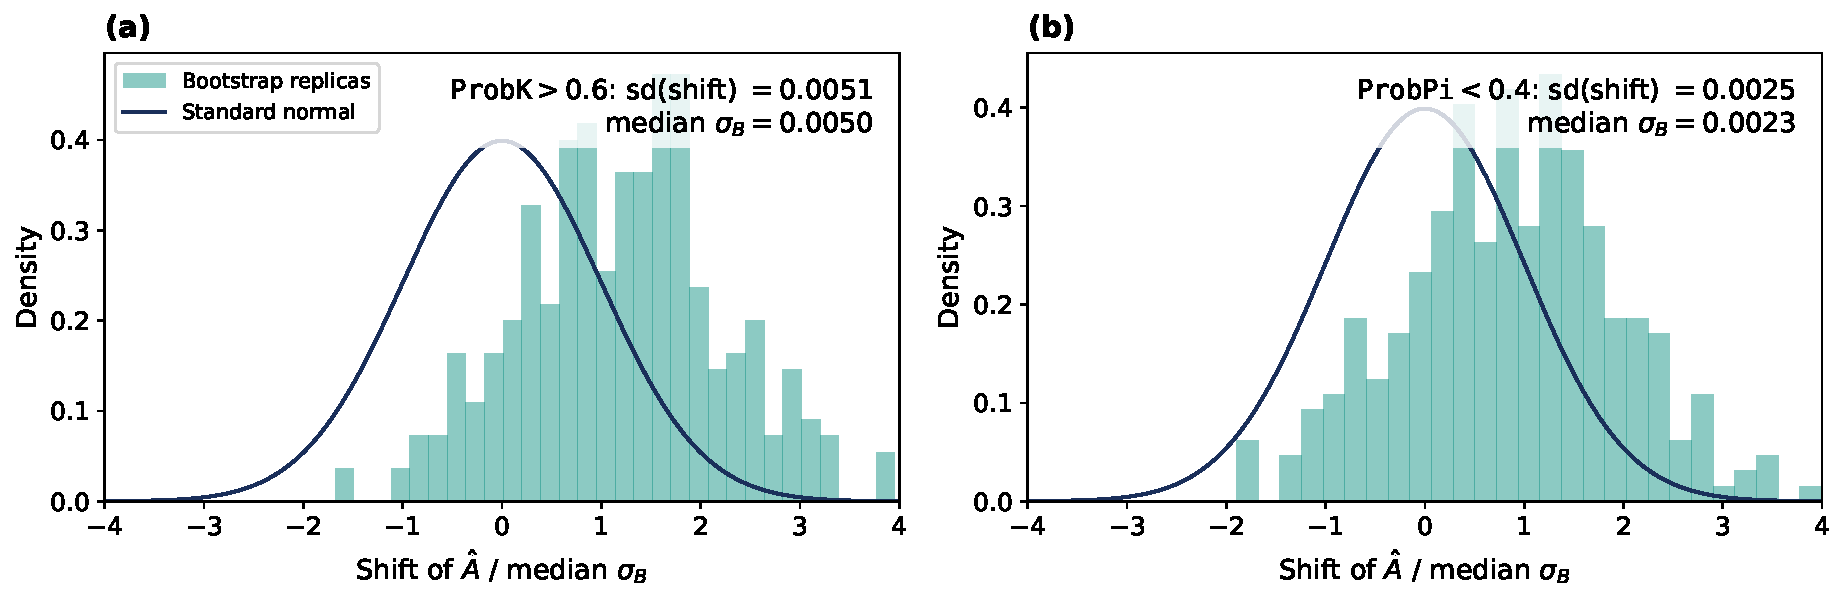
\includegraphics[width=0.95\textwidth]{figures/validation_barlow.pdf}
\caption{Shift of $\hat A$ between the nominal sample and a tighter selection, divided by the median $\sigma_B$, in $300$ bootstrap replicas of the data: (a) $\texttt{ProbK}>0.6$, (b) $\texttt{ProbPi}<0.4$, and standard normal distribution.}
\label{fig:checks_barlow}
\end{figure*}

\subsection{Stability Scans of the Frequentist Fit: Numbers}
\label{sec:freq_stab_numbers}
\emph{In short: the largest shifts are $0.0048$ over the grid of window edges (Fig.~\ref{fig:freq_stability}a) and $0.0126$ over the grid of the two PID cuts (Fig.~\ref{fig:freq_stability}c), whose samples are smaller (mean uncertainty $0.0112$); the signal region moves $\Araw$ by $6\times10^{-5}$ (Fig.~\ref{fig:freq_stability}b).}

Figure~\ref{fig:freq_stability} shows the shift of $\Araw$ with respect to the nominal fit over three grids: (a) the lower and upper edge of the fit window, (b) the lower and upper edge of the signal region, and (c) the lower cut on $\texttt{ProbK}$ and the upper cut on $\texttt{ProbPi}$.

\begin{figure*}[!t]
\centering
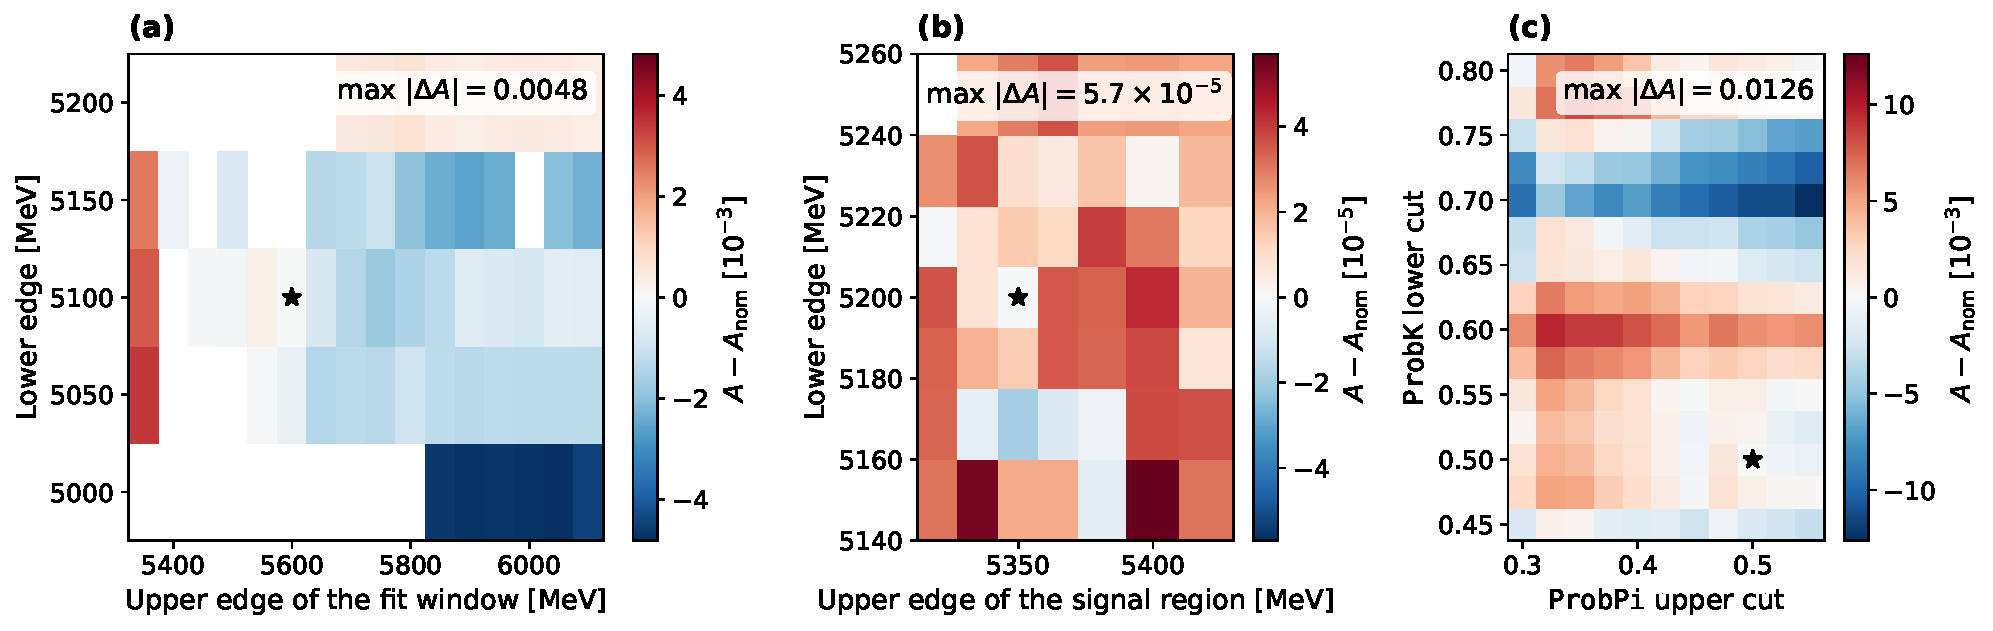
\includegraphics[width=0.95\textwidth]{figures/freq_stability.pdf}
\caption{Stability of the fitted $\Araw$ over the three grids: (a) lower and upper edge of the fit window (only fits with a valid minimum and an accurate covariance are shown); (b) lower and upper edge of the signal region; (c) lower cut on \texttt{ProbK} and upper cut on \texttt{ProbPi}. The colour is the shift with respect to the nominal fit (star), in units of $10^{-3}$ for (a) and (c) and $10^{-5}$ for (b); the statistical uncertainty of the nominal fit is $8.5\times10^{-3}$.}
\label{fig:freq_stability}
\end{figure*}

\section{Comparison of the Two Approaches}
\label{app:ext_comp}
\emph{In short: the profile likelihood against the posterior and the two magnet polarities, the confidence and credible regions in $(A,A_b)$, and the two methods at low statistics.}
\subsection{Profile Likelihood, Posterior and the Two Polarities}
\label{sec:checks_profile}
\emph{In short: profiling and marginalizing the nuisance parameters give the same distribution of $A$ (Fig.~\ref{fig:checks_profile}); the two magnet polarities agree with each other, and combining their likelihoods reproduces the joint fit (Table~\ref{tab:checks_polarity}).}

Table~\ref{tab:checks_polarity} gives $\Araw$ for the two magnet polarities and their combination, by the two methods: the frequentist combination is the sum of the profile likelihoods, the Bayesian one the sequential update of the posterior.

\begin{figure*}[!t]
\makeatletter\def\@captype{table}\makeatother
\centering
\resizebox{\ifdim\width>\linewidth\linewidth\else\width\fi}{!}{\begin{tabular}{lcc}
\toprule
 & Frequentist & Bayesian \\
\midrule
Magnet down & $-0.0492\pm0.0111$ & $-0.0497\pm0.0112$ \\
Magnet up & $-0.0374\pm0.0131$ & $-0.0378\pm0.0129$ \\
Combination of the two & $-0.0443\pm0.0084$ & $-0.0446\pm0.0086$ \\
Joint fit & $-0.0441\pm0.0085$ & $-0.0443\pm0.0085$ \\
\bottomrule
\end{tabular}}
\caption{$\Araw$ for the two magnet polarities and their combination, by the two methods; the frequentist combination is the sum of the profile likelihoods of the two polarities, the Bayesian one the sequential update of the posterior.}
\label{tab:checks_polarity}
\end{figure*}

\subsection{Confidence and Credible Regions in $(A,A_b)$}
\label{sec:checks_region}
\emph{In short: the $68\%$ and $95\%$ regions of the frequentist profile ($\Delta\mathrm{NLL}$ at the $\chi^2_2$ values $2.30$ and $5.99$) and of the Bayesian highest posterior density coincide, and $A=0$ lies outside both (Fig.~\ref{fig:checks_region}).}

Figure~\ref{fig:checks_region} shows the $68\%$ (solid) and $95\%$ (dashed) regions in $(A,A_b)$, frequentist and Bayesian, with the best-fit point and the posterior median.

\begin{figure*}[!t]
\centering
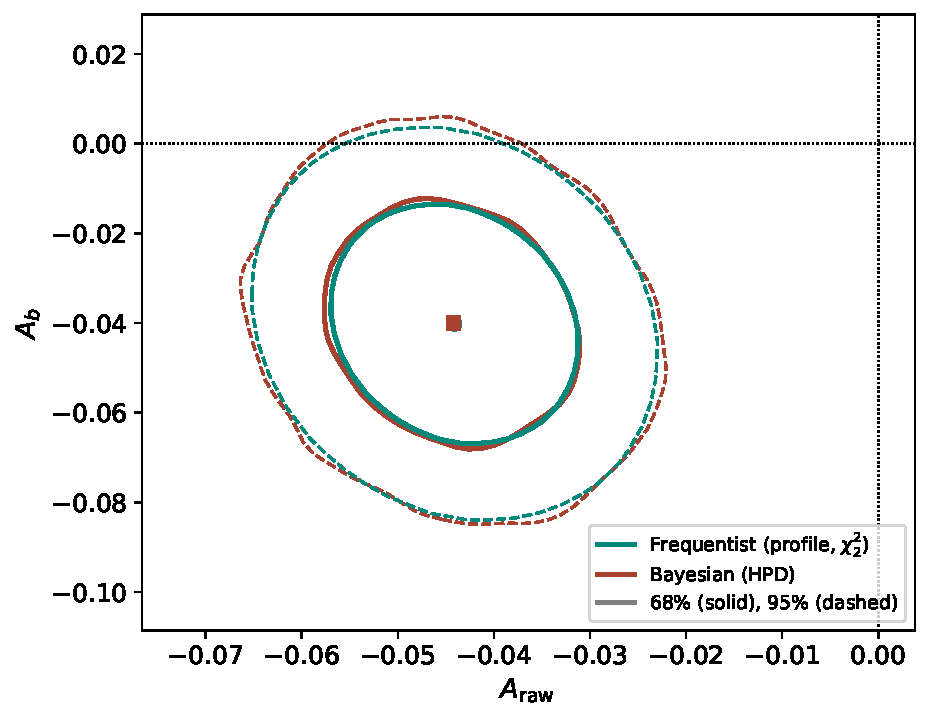
\includegraphics[width=0.5\textwidth]{figures/validation_region_Ab.pdf}
\caption{$68\%$ (solid) and $95\%$ (dashed) regions in $(A,A_b)$: frequentist, from the profile likelihood with $\chi^2_2$ thresholds, and Bayesian, highest-posterior-density regions of the chain. Dots: best-fit and posterior median.}
\label{fig:checks_region}
\end{figure*}

\subsection{Bayesian and Frequentist Intervals at Low Statistics}
\label{sec:bayes_lowstat}
\emph{In short: credible and confidence intervals coincide for $\sim2\times10^4$ candidates with flat priors, and stay equal, in value and coverage, down to $50$ candidates (Fig.~\ref{fig:bayes_lowstat}).}

Figure~\ref{fig:bayes_lowstat} shows the coverage of the $68\%$ (a) and $95\%$ (b) intervals on $A$ against the number of candidates, for the Bayesian credible, the Minos and the Hesse intervals, in $300$ toy-MC datasets per point.

\begin{figure*}[!t]
\centering
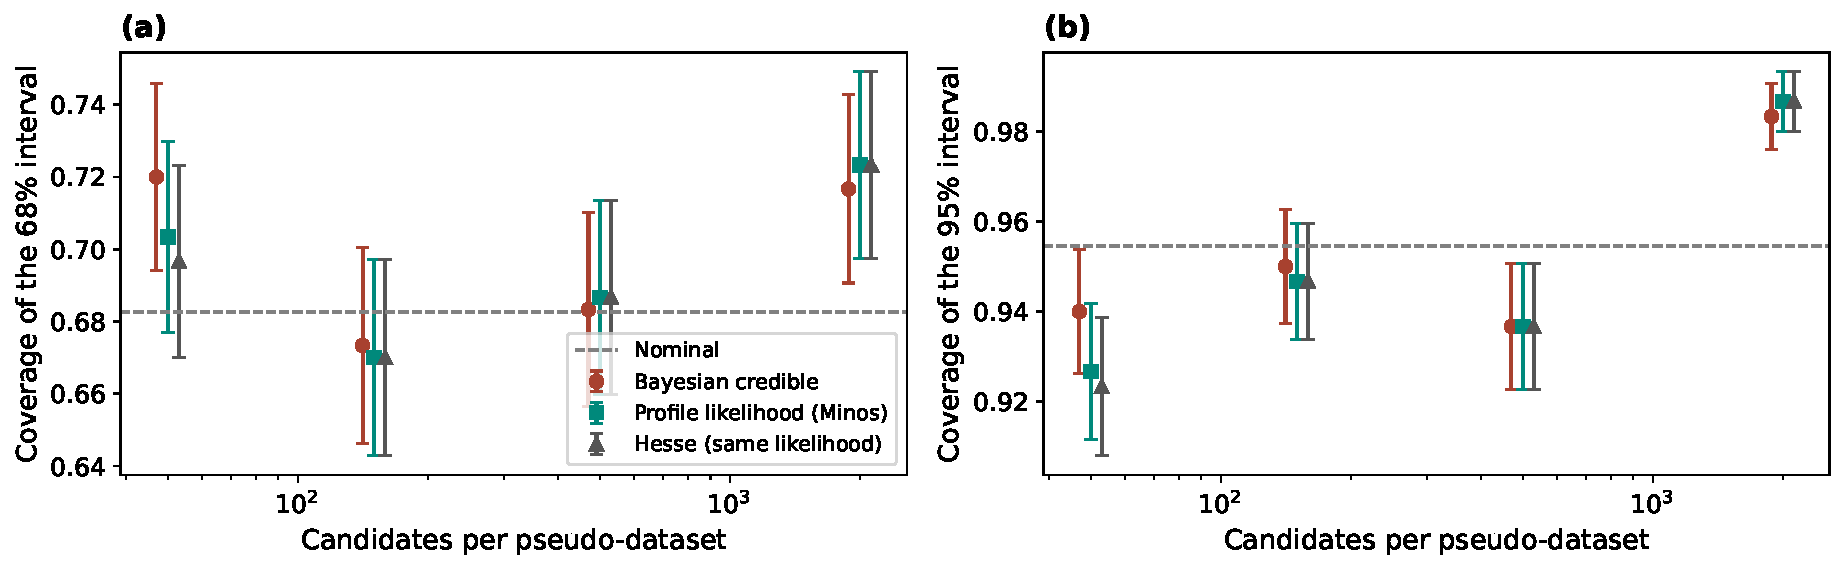
\includegraphics[width=0.95\textwidth]{figures/bayes_nominal_lowstat.pdf}
\caption{Coverage of the (a) 68\% and (b) 95\% intervals on $A$ vs the number of candidates, for the Bayesian credible interval, the profile-likelihood (Minos) interval and the Hesse interval of the same likelihood; 300 toy-MC datasets per point, binomial uncertainties. The dashed lines mark the nominal coverage ($1\sigma$, $2\sigma$; the Bayesian 95\% interval is the 2.5--97.5\% one).}
\label{fig:bayes_lowstat}
\end{figure*}

\FloatBarrier

\section{Notation}
\label{sec:notation}
\emph{In short: the symbols and abbreviations used in the report.}
The symbols used in the text are listed in Table~\ref{tab:notation}.

\begin{table}[h]
\centering
\begin{tabular}{ll}
\toprule
Symbol & \pcell{6.2cm}{Meaning} \\
\midrule
$\Araw$ & \pcell{6.2cm}{raw charge asymmetry $(N^--N^+)/(N^-+N^+)$ of the signal, parameter $A$ of the fit} \\
$\ACP$, $A_P$, $A_D$ & \pcell{6.2cm}{CP asymmetry; production asymmetry of $B^\pm$; detection asymmetry} \\
$A_{\mathrm{count}}$ & \pcell{6.2cm}{counting asymmetry of all candidates of a sample} \\
$A_b$ & \pcell{6.2cm}{asymmetry of the background yields} \\
$N_s$, $N_b$ & \pcell{6.2cm}{signal and background yields (both charges)} \\
$\mu$, $\sigma$ & \pcell{6.2cm}{mean and width of the Gaussian signal} \\
$\lambda_{1,2}^\pm$, $f_\pm$ & \pcell{6.2cm}{slopes and fraction of the double-exponential background, per charge} \\
$\theta$ & \pcell{6.2cm}{vector of the twelve parameters} \\
$\mathcal L$, $\pi$ & \pcell{6.2cm}{likelihood and prior} \\
$q(A)=2\Delta\mathrm{NLL}$ & \pcell{6.2cm}{profile likelihood ratio of $A$; $t(A_{\mathrm{true}})$ at the injected value} \\
$Z$, $p$ & \pcell{6.2cm}{significance and $p$-value of the test of $A=0$} \\
$BF_{01}$, $BF_{10}$ & \pcell{6.2cm}{Bayes factor of $A=0$ against $A$ free, and its inverse} \\
$p_B$ & \pcell{6.2cm}{posterior predictive $p$-value} \\
$\sigma_B$ & \pcell{6.2cm}{expected spread of the shift between nested samples, $\sqrt{|\sigma_{\mathrm{var}}^2-\sigma_{\mathrm{nom}}^2|}$} \\
$N/\tau$ & \pcell{6.2cm}{chain length in integrated autocorrelation times} \\
$S_i$, $S_k$ & \pcell{6.2cm}{local significance of a Dalitz bin or cluster with respect to the global asymmetry} \\
\bottomrule
\end{tabular}
\caption{Main symbols used in the text.}
\label{tab:notation}
\end{table}

\FloatBarrier

